% CABECERA DESCRIPCIÓN
% BEGIN_FOLD
%%%%%%%%%%%%%%
% Fichero: uclmTFGesi.tex
% Autor: Jesús Salido Tercero (https://www.esi.uclm.es/www/jsalido)
% Fecha (creación): febrero 2010 
% Rev. : marzo 2024
% Descripción: Plantilla para memoria de TFG 
% (Escuela Sup. de Informática, UCLM). Creada para el curso 
% “LaTeX esencial para preparación de TFG, Tesis y otros documentos 
% académicos” (Esc. Sup. Informática-UCLM)
%
%### Compilación 
%
% Esta plantilla ha sido preparada para compilarse con `pdflatex`  
% (bibliografía con `bibtex`).
%$ $
% Para su compilación se aconseja utilizar `latexmk` (requiere para su 
% ejecución de un intérprete perl:
%
%> \$> latexmk -gg -pdf -bibtex-cond1 -quiet -outdir=build uclmTFGesi.tex
%
% Para la automatización del trabajo con esta plantilla es recomendable el 
% empleo de IDE dedicados como [TeXstudio](https://www.texstudio.org/).
%
% Una versión revisada de esta plantilla está disponible en overleaf.
% Puede crearse un proyecto propio para escribir un TFG directamente en 
% overleaf, o bien descargarla como un archivo .zip para su utilización en 
% modo local.
%
% Si deseas acceder a la versión de desarrollo puedes encontrarla en GitHub:
%	https://github.com/JesusSalido/TFG_ESI_UCLM
%%%%%%%%%%%%%%
% END_FOLD

\documentclass[ 		% Clase del documento
	11pt,				% Tamaño de letra
	a4paper,			% Tamaño de papel
	twoside,			% Impresión a doble cara
	openright,			% La apertura de cap. a la dcha.
%	draft       		% Versión borrador (sin figuras)
	final       		% Versión final
]{book}

%--- Márgenes del documento
\usepackage[top=2.5cm,    % Superior
            bottom=2.5cm, % Inferior
            inner=3.5cm,  % Interior 
            outer=2cm     % Exterior
]{geometry}

\pdfcompresslevel=0
\pdfobjcompresslevel=0
\pdfoptionpdfminorversion=6 % Elimina warnings

\newif\ifspanish\spanishtrue
% OPT.: Idioma pral. inglés, descomentar
%\spanishfalse
 
\newif\ifpageonfooter\pageonfooterfalse
% OPT: nº pág. en el pie de página, descomentar
%\pageonfootertrue

%=== PAQUETE QUE ACOMPAÑA A LA PLANTILLA
%--- Paquetes empleados por la plantilla
\usepackage{uclmTFGesi} % Carga de paquetes en background
%===

% OPT: Nivles de índice y numeración de secciones
\setcounter{tocdepth}{1} % Suprime del índice los apdos. de nivel mayor
\setcounter{secnumdepth}{3} % Suprime numeración de secciones de nivel mayor

% OPT: Opciones de hipertexto
\hypersetup{% (Metadatos del fichero PDF generado)
	breaklinks=true,         % Enlaces con división entre líneas
    linktocpage=true,        % T/F=enlace al nº de pág./texto completo
	colorlinks=true,         % T/F=texto en color/recuadro al texto
%    hidelinks,               % Oculta colores en los enlaces (en negro)
    linkcolor=UCLMred,       % Color links internos
    anchorcolor=UCLMred,     % Color para anclas a texto
	urlcolor=aquaESI,        % Color para URL enlazadas
	citecolor=UCLMred,       % Color para citas a bibliografía
	bookmarksopen=true,      % Abre PDF con panel de marcadores abierto
	bookmarksnumbered=true,  % Incluye números en marcadores
	pdftoolbar=true,         % Muestra la toolbar de Acrobat
	pdfmenubar=true,	     % Muestra la menubar de Acrobat
}

%---
% OPT.: Citación APA, descomentar
% Permite citación (Autor, año) y bibliografía APA
%\usepackage[natbibapa]{apacite} 
%---

%% ============================
%% Añade aquí los paquetes y comandos adicionales que necesites
%% ===>



% -------------------------
% -------------------------
% -------------------------
% BEGIN_FOLD
% -------------------------
% -------------------------
% -------------------------
% EDITA: Datos del documento. 
% Definición de variables empleadas en el documento por lo que no son
% traducidos. Cuando algún campo puede tener varias líneas aparecen dos
% campos señalados como <campo>Primera y <campo>Segunda. Si no se desea 
% emplear los campos opcionales (OPT.) estos deben comentarse.
% -------------------------
\tituloPrimera{Plantilla guía de TFG para la ESI-UCLM} % 1ª Línea
\tituloSegunda{Curso de {\LaTeX{}} esencial} % OPT.: Títulos largos.
\tituloCorto{Plantilla guía de TFG} % Título corto (mostrado en pág. de 
%créditos)
\autor{Jesús Salido Tercero}
\email{jesus.salido@uclm.es}					
\instEdu{UNIVERSIDAD DE CASTILLA-LA MANCHA}
\centroEdu{ESCUELA SUPERIOR DE INFORMÁTICA}
\titulacion{GRADO EN INGENIERÍA INFORMÁTICA} 
% (EN: BACHELOR IN COMPUTING ENGINEERING)
\tipoDoc{TRABAJO FIN DE GRADO} % (EN: BACHELOR DISSERTATION)
% Si las fechas se desean en inglés hay que ponerla explícita.
\mesTF{julio}        	% Mes de defensa (incluir siempre)
\monthTF{July}        	% En inglés (incluir siempre)
\yearTF{2024}        	% Año de defensa
\cityTF{Ciudad Real}	% Ciudad de defensa


\makeatletter
\hypersetup{% (Metadatos del fichero PDF generado)
	pdftitle={\@title},      % Título
	pdfauthor={\@author},    % Autor
	pdfsubject={\@tipoDoc}   % Tipo de de documento
}
\makeatother

% OPT: Logo institución
% Fichero con escudo de la institución (en directorio ./figs)
% Logo de la ESI (consulta obligatoriedad de uso concreto)
\escudo{esiLogo} % Logo centro (imagen corporativa). Fichero gráfico (pdf, 
%png o jpg)
% -------------------------
% -------------------------
% -------------------------
% END_FOLD


% -------------------------
% -------------------------
% -------------------------
% -------------------------
%
% CUERPO del documento
%
% -------------------------
\begin{document}
%--- PORTADAS + FRONTMATTER
% BEGIN_FOLD
% OPT.: Ficheros incluidos, modifica o comenta.
\frontmatter
\pagestyle{empty}  % Páginas sin cabecera ni pies
% OJO: Editar este fichero a voluntad para ajustarlo al resultado deseado.
% OJO: Poner especial atención en usar los adjetivos de género correctos.
% -------------------------
% -------------------------
% -------------------------
% PORTADAS: (Incluidas páginas para créditos y dedicatoria)
% -------------------------
% -------------------------------------------------------------------------
% -------------------------------------------------------------------------
% -------------------------------------------------------------------------
% PORTADA PRAL. (1)
% Puedes incluir directamente la portada realizada por un programa externo.
% Y directamente modificar el diseño que se proporciona. 
% NOTA: Para eliminar líneas sin alterar el espaciado original se recomienda emplear \phantom{text}
\begin{titlepage}
    \makeatletter
	\begin{center}
        \pdfbookmark{Portada}{portada}
        \vspace{1cm}
		\includegraphics[width=4.5cm]{\@escudo}\vspace{1cm} 
		
		{\LARGE \textbf{\@instEdu\\[0.5ex]
				\@centroEdu\\[2cm]
				\@titulacion}}\\[0.5cm]
        {\large \textbf{Tecnología específica de computación}}\\[1.5cm]
        % (EN: Specialization in ...)
		{\LARGE \textbf{\@tipoDoc}}\\[1cm]	
		{\LARGE \@tituloPrimera}\\ \smallskip%			
		\ifdefined\@tituloSegunda{\LARGE \@tituloSegunda}\\[3cm]
		\else \phantom{\LARGE	Texto fantasma}\\[3cm]
		\fi
		{\Large \@autor}\vfill%
	\end{center}
	
	\begin{flushright}
		{\Large \ifspanish \@mesTF \else \@monthTF \fi, \@yearTF}
	\end{flushright}
	
%	\cleardoublepage
    \makeatother
\end{titlepage}






% -------------------------------------------------------------------------
% -------------------------------------------------------------------------
% -------------------------------------------------------------------------
% PORTADA INTERIOR (2)
% Puedes incluir directamente la portada realizada por un programa externo.
% Y directamente modificar el diseño que se proporciona. 
% NOTA: Para eliminar líneas sin alterar el espaciado original se recomienda emplear \phantom{text}
\begin{titlepage}
    \makeatletter
	\begin{center}
        \vspace{1cm}
		\includegraphics[width=4.55cm]{\@escudo}\vspace{1cm}
		
		{\LARGE \textbf{\@instEdu \\[0.5ex]
				\@centroEdu}}\\[0.5cm]
		{\Large \textbf{Departamento de tecnologías}}\\ \smallskip%
        {\Large\textbf{y sistemas de información}}\\[0.5cm]
		{\large \textbf{Tecnología específica de computación}}\\[1.5cm]
%		(EN: Specialization in ...)
		{\LARGE \textbf{\@tipoDoc}}\\[1cm]
		
		
		{\LARGE \textbf{\@tituloPrimera}}\\ \smallskip%		
		\ifdefined\@tituloSegunda{\LARGE \textbf{\@tituloSegunda}}
		\else \phantom{\LARGE Texto fantasma}
		\fi
	\end{center}
	\vfill%
	\begin{flushleft}
		{\Large Autor: \@autor} \\ \bigskip% (EN: Author)
		{\Large Tutor: Luis Jiménez Linares} \\ \bigskip% (EN: Co-Supervisor)
		%{\Large Co-tutor(a): nombre y apellidos}
	\end{flushleft}
	\vspace{2cm}%
	\begin{flushright}
		{\Large \ifspanish \@mesTF \else \@monthTF \fi, \@yearTF}
	\end{flushright}
	\cleardoublepage
    \makeatother
\end{titlepage}
	




% -------------------------------------------------------------------------
% -------------------------------------------------------------------------
% -------------------------------------------------------------------------
% OPT.: CRÉDITOS (aunque no es obligatorio es recomendable).
% -------------------------
%
% CRÉDITOS
%
% -------------------------
% Esta es una página reservada para señalar información relativa a los derechos de autor y la licencia de distribución y uso del documento. Esta página debería ser aprovechada también para informar de cualquier tipo de cesión de los derechos anteriormente citados. El autor del TFG debe tener presente que el incumplimiento de la legislación vigente en materia de protección de la propiedad intelectual es de su exclusiva responsabilidad independientemente de la cesión de derechos que este haya convenido para su obra ya que no son objeto de cesión aquellos derechos de los que no se es poseedor.


\ifspanish
	\selectlanguage{spanish}% Emplea idioma español
\else
	\selectlanguage{english}% Emplea idioma inglés
\fi
\null\vspace{6cm}
\makeatletter
{\pdfbookmark[1]{Créditos}{creditos}\small \noindent \@tituloCorto\\
\textcopyright{} \@autor, \@yearTF\\[1cm]
% EDITA: El autor puede elegir el tipo de licencia que desee para 
%distribuir su TFG que puede variar con respecto a la de este documento en 
%el que si permitimos obra derivada para que no surjan dudas sobre la 
%reutilización del material.
Este documento se distribuye con licencia CC BY-NC-SA 4.0. El texto 
completo de la licencia se puede obtener en 
\url{https://creativecommons.org/licenses/by-nc-sa/4.0/}.
\makeatother

La copia y distribución de esta obra está permitida en todo el mundo, sin regalías y por cualquier medio, siempre que esta nota sea preservada. Se concede permiso para copiar y distribuir traducciones de este libro desde el español original a otro idioma, siempre que la traducción sea aprobada por el autor del libro y tanto el aviso de copyright como esta nota de permiso, sean preservados en todas las copias.


\vfill
% NOTA: Por favor, deja esta nota de atribución al uso de la plantilla LaTeX.
Este texto ha sido preparado con la plantilla \LaTeX{} para Trabajo Fin de 
Estudios en Ingeniería Informática para la UCLM publicada por 
\href{https://www.esi.uclm.es/www/jsalido}{Jesús Salido} en el repositorio 
público Zenodo, DOI: 
\href{https://doi.org/10.5281/zenodo.4561708}{10.5281/zenodo.4561708}, como 
parte del curso 
\href{http://visilab.etsii.uclm.es/?page_id=1468}{\emph{<<\LaTeX{} esencial 
para preparación de TFG, tesis y otros documentos académicos>>}} impartido 
en la Escuela Superior de Informática de la Universidad de Castilla-La 
Mancha. Si la empleas para preparar tu TFG, te agradeceré que la 
cites~\cite{salido19} e incluyas en tus referencias como se indica en 
Zenodo con el DOI suministrado para todas las versiones.}

\noindent 
\includegraphics[width=0.15\linewidth]{by-nc-sa}

\cleardoublepage

% NOTA: Para citar este documento empleando bibtex puedes emplear el registro siguiente:
%@www{salidoTFG,
%  author       = {Jesús Salido},
%  title        = {Plantilla guía de TFG para la ESI-UCLM},
%  year         = {2019},
%  editor       = {GitHub},
%  organization = {Universidad de Castilla-La Mancha},
%  url          = {https://github.com/JesusSalido/TFG_ESI_UCLM},
%  doi          = {10.5281/zenodo.4574562}
%}


%---



%---




% -------------------------------------------------------------------------
% -------------------------------------------------------------------------
% -------------------------------------------------------------------------
% CALIFICACIÓN TRIBUNAL
% Puedes incluir directamente la portada realizada por un programa externo.
%---
\begin{titlepage}
    \pdfbookmark[1]{Tribunal}{tribunal}
 %   \makeatletter
	{\flushright \LARGE \textsc{Tribunal:}}
	
	\vspace*{\stretch{0.5}}
	\hspace*{1cm}{\Large Presidente: \hrulefill}
	
	\vspace*{\stretch{0.5}}
	\hspace*{1cm}{\Large Vocal: \hrulefill}
	
	\vspace*{\stretch{0.5}}
	\hspace*{1cm}{\Large Secretario(a): \hrulefill}
	
	\vspace*{\stretch{0.5}}
	{\flushright \LARGE \textsc{Fecha de defensa:} \hrulefill}
	
	\vspace*{\stretch{1.5}}
	{\flushright \LARGE \textsc{Calificación:} \hrulefill}
	
	\vspace*{\stretch{2.5}}
	\begin{center}
		\begin{tabularx}{\linewidth}{X X X}
			{\large \textsc{Presidente}} & {\large \textsc{Vocal}} & {\large \textsc{Secretario(a)}}\\[2.5cm]
			Fdo.: & Fdo.: & Fdo.:		
		\end{tabularx}
	\end{center}
	\cleardoublepage
%    \makeatother
\end{titlepage}



% -------------------------------------------------------------------------
% -------------------------------------------------------------------------
% -------------------------------------------------------------------------
% OPT.: DEDICATORIA (1 pág. máximo) comentar si no se desea incluir.
% Aunque opcional, no se debería perder la oportunidad de poder 
% dedicar el trabajo a alguien MUY especial. Debe ocupar como mucho dos líneas
% (no confundir con los agradecimientos).
% EDITAR: Dedicatoria.

\null\vspace{\stretch{1}}
\begin{flushright}
\emph{A mi familia \\ % A alguien muy especial
Por su apoyo incondicional}
\end{flushright}
\vspace{\stretch{2}}\null
\cleardoublepage


%---
%
% FIN PORTADAS: 
% |
% |
% -> ---------------------- % Diseño de portadas
%\input{./preambulo/PortadaETSII} % Por ej.,: Otras portadas
%\includepdf{fichero_portada.pdf} % Incluso como fichero PDF

%--- Ajustes del documento.
\pagestyle{plain}	% Páginas sólo con numeración inferior al pie

% -------------------------
%
% RESUMEN:
% 
%

% EDITAR: Resumen (máx. 1 pág.)
%\cleardoublepage % Se incluye para modificar el contador de página antes de añadir bookmark
\phantomsection  % Necesario con hyperref
\addcontentsline{toc}{chapter}{Resumen} % Añade al TOC.
\selectlanguage{spanish} % Selección de idioma del resumen.
\makeatletter
\begin{center} %
   {\textsc{TRABAJO FIN DE GRADO - ESCUELA SUPERIOR DE INFORMÁTICA 
   (UCLM)}\par} % Tipo de trabajo
   \vspace{1cm} %  
   {\textbf{\Large\@tituloCorto}\par}  % Título del trabajo
   \vspace{0.4cm} %
   {\@autor \\ \@cityTF,{} \@mesTF{} \@yearTF\par} 
   \vspace{0.9cm} %
   {\textbf{\large\textsf{Resumen}}\par} % Título de resumen
\end{center}   
\makeatother %
En una página como máximo, el resumen explica de modo conciso la problemática que trata de resolver el trabajo \emph{(<<Qué>>)}, la metodología para  abordar su solución (\emph{<<Cómo>>)} y las principales conclusiones del trabajo. En los trabajos cuyo idioma principal sea el inglés, el orden de \textsf{Resumen} y \textsf{Abstract} se invertirá. 

En concreto este documento debe servir como guía para preparar, con \LaTeX, el TFG en la \href{http://webpub.esi.uclm.es/}{Escuela Superior de Informática} (ESI) de la Univ. de Castilla-La Mancha (UCLM), siguiendo la \href{https://pruebasaluuclm.sharepoint.com/sites/esicr/tfg/SitePages/Inicio.aspx}{normativa de aplicación}. Está disponible tanto en \href{https://github.com/JesusSalido/TFG_ESI_UCLM}{GitHub} como \href{https://www.overleaf.com/latex/templates/plantilla-de-tfg-escuela-superior-de-informatica-uclm/phjgscmfqtsw}{Overleaf}. Por tanto, se puede emplear, tanto en un equipo con \LaTeX{} (modo local) instalado, o bien empleando el servicio de edición \href{https://www.overleaf.com/latex/templates/plantilla-de-tfg-escuela-superior-de-informatica-uclm/phjgscmfqtsw}{Overleaf} (modo online).

Este texto se aprovecha para proporcionar información sobre la elaboración de la memoria del TFG con ayuda de \LaTeX{} empleando este documento como plantilla. Por este motivo, sigue una estructura similar a la que se espera encontrar en un TFG, mostrando ejemplos de uso de distintos elementos y comandos de maquetación de textos que se amplía en el anexo~\ref{cap:AnexoA}.

\noindent\emph{IMPORTANTE: Aunque la plantilla se ajusta a las necesidades y reglamentación de la ESI-UCLM, se puede adaptar fácilmente a otras titulaciones, instituciones y otros documentos de carácter académico. Esta plantilla permite la elaboración automática del documento en idioma inglés en cualquier SO (Windows, Linux, Mac OSX, etc.).}

\bigskip
\noindent\textbf{Palabras clave}: TFG, \LaTeX, plantilla, UCLM \emph{(como mucho 5 palabras que se puedan emplear como etiquetas de búsqueda)}.

%---
\cleardoublepage % Se incluye para modificar el contador de página antes de añadir 





% EDITAR: Abstract (máx. 1 pág.)
%---
\phantomsection  % Necesario con hyperref
\addcontentsline{toc}{chapter}{Abstract} % Añade al TOC.
\selectlanguage{english} % Selección de idioma del resumen.
\makeatletter
\begin{center} %
   {\textsc{BACHELOR DISSERTATION - ESCUELA SUPERIOR DE INFORMÁTICA 
   (UCLM)}\par}
   \vspace{1cm} %  
   {\textbf{\Large Guided template for TFG}\par}
   \vspace{0.4cm} %
   {\@autor \\ \@cityTF,{} \@monthTF{} \@yearTF\par} 
   \vspace{0.9cm} %
   {\textbf{\large\textsf{Abstract}}\par} 
\end{center}   
\makeatother %
\emph{English version for the abstract.}

\bigskip 

\noindent\textbf{Keywords}: \dots

\cleardoublepage % Se incluye para modificar el contador de página antes de añadir 

 % Resumen/Abstract
% Selección del idioma principal del texto
\ifspanish
	\selectlanguage{spanish}
\else
	\selectlanguage{english}
\fi

% EDITAR: Según el gusto del usuario

% -------------------------
%
% AGRADECIMIENTOS (recomendable máx. 1 pág.)
%
% -------------------------
\phantomsection % Necesario con hyperref
\chapter*{Agradecimientos} % Opción con * para que no aparezca en TOC ni numerada
\addcontentsline{toc}{chapter}{Agradecimientos} % Añade al TOC.

 Aunque es un apartado opcional, haremos bueno el refrán \emph{<<es de bien nacidos, ser agradecidos>>} si empleamos este espacio como un medio para agradecer a todos los que, de un modo u otro, han hecho posible que el trabajo realizado \emph{llegue a buen puerto}. Esta sección es ideal para agradecer a directores, profesores, mentores, familiares, compañeros, amigos, etc. 
 
 Estos agradecimientos pueden ser tan personales como se desee e incluir anécdotas y chascarrillos, pero recuerda que \emph{no deberían ocupar más de una página}.

\makeatletter		
\begin{flushright}
	\vspace{1,5cm}
	\textit{\@autor}\\
	\@cityTF, \@yearTF
\end{flushright}
\makeatother % Agradecimientos etc.

% -------------------------
%
% -NOTACIÓN: Lista de símbolos con significado especial.
%
% -------------------------
\cleardoublepage
\phantomsection % Necesario con hyperref

% El método mostrado en este fichero es un modo rápido de incluir nomeclatura y listade acrónimos. En trabajos donde se precise un trabajo más depurado e intensivo puede recurrirse a los paquetes:
%   - nomencl
%   - acronym

\chapter*{Notación y acrónimos} % Opción con * para que no aparezca en TOC ni numerada
\addcontentsline{toc}{chapter}{Notación y acrónimos} % Añade al TOC.

\section*{Notacion}
Ejemplo de lista con notación (o nomenclatura) empleada en la memoria del TFG.\footnote{Se incluye únicamente con propósito de ilustración, ya que el documento no emplea la notación aquí mostrada.}

\begin{tabular}{r r p{0.8\linewidth}}
$A, B, C, D$	& : & Variables lógicas \\
$f, g, h$		& :	& Funciones lógicas \\
$\cdot$			& : & Producto lógico (AND), a menudo se omitirá como en $A 
B$ en lugar de $A \cdot B$\\
$+$				& : & Suma aritmética o lógica (OR) dependiendo del 
contexto\\
$\oplus$		& : & OR exclusivo (XOR)\\
$\overline{A}$ o ${A}'$	& : & Operador NOT o negación
\end{tabular}

\section*{Lista de acrónimos}
% OJO: Esta lista debería estar ordenada alfabeticamente (hacer de modo manual).
Ejemplo de lista \emph{ordenada alfabéticamente} con los acrónimos empleados en el texto.\footnote{Se pueden omitir aquellos acrónimos que son reconocidos en el contexto académico (p.~ej., PhD), aunque aquí se han incluido a efectos ilustrativos.}

\begin{tabular}{r r p{0.8\linewidth}}
CASE& : &Computer-Aided Software Engineering \\
CTAN& : &Comprenhensive \TeX{} Archive network \\
IDE& : &Integrated Development Environment \\
ECTS& : &European Credit Transfer and Accumulation System \\
OOD& : &Object-Oriented Design \\
PhD& : &Philosophiae Doctor \\
RAD& : &Rapid Application Development \\
SDLC& : &Software Development Life Cycle \\
SSADM& : &Structured Systems Analysis \& Design Method \\
TFE& : &Trabajo Fin de Estudios \\
TFG& : &Trabajo Fin de Grado \\
TFM& : &Trabajo Fin de Máster \\
UML& : &Unified Modeling Language
\end{tabular} % [OPT:] Notación empleada.
% -------------------------
%
% ÍNDICES: 
% EDITAR: Si alguno de los índices no existe, su inclusión se puede comentar.
%
% -------------------------
\setindexnames % Ajusta nombres (sólo en español).
\pagestyle{fancy} % Estilo de página ajustado por fancyhdr

%--- Índice general
\cleardoublepage
\phantomsection % Necesario con hyperref
\pdfbookmark[0]{Índice general}{idx_toc}% idx_toc.0 % Bookmark en PDF
\tableofcontents  % Índice general
% Todos los listados se han incluido en el índice gral. de contenidos. De 
%modo automático también quedan añadidos a los bookmarks del PDF. Si se 
%desean 
%eliminiar del TOC se pueden comentar el comando \addcontensline.
%---

%--- Índice de figuras
\cleardoublepage
\phantomsection % Necesario con hyperref
\addcontentsline{toc}{chapter}{\listfigurename} % Añade la lista de figuras al TOC (también a bookmarks en PDF)
%\pdfbookmark[0]{\listfigurename}{idx_lof}% idx_lof.0 % Bookmark en PDF
\listoffigures    % Índice de figuras (opcional)
%---

%--- Índice de tablas
\cleardoublepage
\phantomsection % Necesario con hyperref
\addcontentsline{toc}{chapter}{\listtablename} % Añade la lista de tablas al TOC (también a bookmarks en PDF)
%\pdfbookmark[0]{\listtablename}{idx_lot}% idx_lot.0 % Bookmark en PDF
\listoftables % Índice de tablas (opcional)
%---

%--- Índice de listados
% Comentar todo el bloque para no incluir.
\cleardoublepage
\phantomsection % Necesario con hyperref
\addcontentsline{toc}{chapter}{\lstlistlistingname} % Añade la lista de listados al TOC (también a bookmarks en PDF)
%\pdfbookmark[0]{\lstlistlistingname}{idx_lol}% idx_lol.0 % Bookmark en PDF
\lstlistoflistings % Índice de listados creados con listings (opcional)
%---

%--- Índice de algoritmos
% Comentar todo el bloque para no incluir.
\cleardoublepage
\phantomsection % Necesario con hyperref
\addcontentsline{toc}{chapter}{\listalgorithmcfname} % Añade la lista de algoritmos al TOC (también a bookmarks en PDF)
%\pdfbookmark[0]{\listalgorithmcfname}{idx_loa}% idx_loa.0 % Bookmark en PDF
\listofalgorithms % Índice de algoritmos creados con algortihm2e
%---

 % Índice de contenido, figuras, tablas, listados, etc.
% END_FOLD
%--- (FIN FRONTMATTER)



% -------------------------
% -------------------------
% -------------------------
% -------------------------
%
%--- MAINMATTER
% Capítulos del documento
\savepagecnt % Se almacena en un contador interno el nº de páginas actual
% Debe ir antes de \mainmatter (antes de que se reinicie el cnt page)
\mainmatter
% Justo antes del primer capítulo del libro. Activa la numeración con números arábigos y reinicia el contador de páginas.

% Ajusta valor de cabeceras y pies a comienzo de capítulo
\ifpageonfooter
\else
	\cleanhdfirst
\fi

% Reajuste del n. de pág. consecutivo para no reiniciar pag. en Cáp. 1
%\contpagination % Comentado para reiniciar paginación (pag. 1)
% -------------------------
% --- CAPÍTULOS: Un fichero por capítulo.
% -------------------------
% puedes emplear los comandos señalados (proporcionados por paquete 
%`setspace')
% OPT: Interlineado de una línea (por defecto)
%\onehalfspacing % Ajusta interlineado a 1.5 líneas

% OPT.: Ficheros incluidos correspondientes a los caps.
\chapter{Introducción}
\label{cap:Introduccion}

\section{Contexto}

La tecnología de simuladores ha crecido de manera importante, llevando estas herramientas de simples representaciones a sistemas complejos que replican con alta precisión las condiciones reales de diversos entornos. En particular, los simuladores deportivos han encontrado un nicho significativo en el entrenamiento y desarrollo de habilidades en disciplinas como la conducción deportiva, conocida popularmente como Simracing. Estos simuladores permiten a los pilotos experimentar una conducción casi real, utilizando hardware especializado, como volantes y asientos, junto con software que reproduce las pistas y las leyes físicas involucradas, todo ello a un coste mucho menor comparado con el entrenamiento en pistas reales. El mundo del Simracing está dominado por varias plataformas de simulación, cada una con sus características propias, ventajes e inconvenientes. Entre las más reconocidas se encuentran iRacing \cite{iRacing}, Assetto Corsa \cite{AssetoCorsa}, RFactor \cite{rFactor} y Gran Turismo \cite{granTurismo}. iRacing, en particular,  destaca no sólo por su realismo y precisión, sino también por disponer de una comunidad activa y extensa, base de recursos para desarrollo y análisis de datos. Su realismo en la física de conducción, la variedad de vehículos y pistas, y el soporte continuo lo convierten en una de las opciones preferidas tanto por pilotos aficionados como profesionales.

\section{Análisis de la telemetría}

El análisis de telemetría es crucial para el entrenamiento en Simracing. Las plataformas como iRacing permiten extraer archivos de telemetría que capturan detalladamente los datos de la simulación, permitiendo a los pilotos y entrenadores identificar áreas de mejora. iRacing ofrece la opción de respaldar los archivos de telemetría cuando el jugador lo activa. Esta funcionalidad registra, a una frecuencia predeterminada de 60 Hz, variables como la velocidad, el porcentaje de freno, el ángulo de giro del volante, entre otros. Estas variables se registran con la frecuencia indicada, proporcionando el conjunto de datos necesario para realizar un análisis detallado y preciso del desempeño del piloto.
Para este proyecto, se ha seleccionado el formato .ibt de iRacing debido a su amplio uso y la riqueza de datos que proporciona, ideal para el análisis detallado y la extracción de métricas clave, necesarias para la mejora del rendimiento en Simracing.
Actualmente, la mayoría de las herramientas avanzadas para el análisis de estos datos son de pago, lo cual puede limitar el acceso a usuarios que no pueden permitirse estas soluciones costosas. Herramientas como Motec \cite{motec}, Atlas \cite{atlas} y Virtual Racing School \cite{vrs} ofrecen análisis profundos y detallados, pero su coste puede ser prohibitivo para muchos entusiastas del Simracing.
El análisis de telemetría implica la recolección y procesamiento de grandes cantidades de datos generados durante las sesiones de entrenamiento y competencia. Estos datos incluyen, pero no se limitan a, velocidades, fuerzas G, ángulos de dirección, uso de frenos y acelerador, entre otros. La capacidad de interpretar estos datos de manera eficaz puede marcar la diferencia entre un piloto promedio y uno de élite. Sin embargo, la interpretación requiere herramientas avanzadas que puedan procesar la información de manera rápida y precisa, además de presentarla en un formato accesible y comprensible.


\section{Motivación}

El principal motor de este proyecto es desarrollar una herramienta de análisis de telemetría de código abierto para Simracing, específicamente enfocada en la plataforma iRacing. Esta herramienta tiene como objetivo ofrecer una alternativa libre a las actuales soluciones de pago, facilitando el acceso a un análisis de telemetría avanzado a una mayor comunidad de usuarios y fomentando la colaboración comunitaria. Al ser de código abierto, permitirá a los usuarios implementar técnicas de análisis y utilizar métricas que consideren relevantes, superando las limitaciones de los productos privativos que no pueden ser extendidos fácilmente.
Además de democratizar el acceso a tecnologías avanzadas de análisis, este proyecto pretende impulsar la innovación dentro de la comunidad de Simracing. Los productos de análisis privativos suelen ser cerrados y limitados en términos de extensión, lo que puede ser una barrera para pilotos y equipos que deseen aplicar nuevas técnicas de análisis de datos o integrar métricas personalizadas.
Como parte de este proyecto, también se contempla la creación de un sistema de recomendación de acciones en lenguaje natural. Este sistema proporcionará indicaciones claras y precisas sobre las mejoras que el piloto debe realizar, basándose en el análisis detallado de la telemetría. De esta manera, se pretende no sólo facilitar el análisis de datos, sino también traducir dicho análisis en recomendaciones concretas y accionables para optimizar el rendimiento del piloto.


\section{Impacto del proyecto}

Para la comunidad de Simracing, el proyecto ofrece una herramienta poderosa y accesible que puede transformar la forma en que los pilotos analizan y mejoran su rendimiento. Al ser de código abierto, la herramienta no solo democratiza el acceso a tecnologías avanzadas de análisis, sino que también fomenta la innovación y el desarrollo continuo, permitiendo a los usuarios adaptar y mejorar la herramienta de acuerdo con sus necesidades específicas.
Además, la implementación de un sistema de recomendación de acciones en lenguaje natural puede tener un impacto significativo en la computación y en el desarrollo de sistemas recomendadores. Este enfoque no solo facilita la interpretación de los datos por parte de los pilotos, sino que también sirve como un caso de estudio para la aplicación de técnicas de agrupamiento, como K-means o \ac{fcm} en entornos dinámicos y complejos.
El proyecto también tiene el potencial de influir positivamente en la ciencia y la academia, proporcionando un recurso valioso para la investigación y la enseñanza en áreas relacionadas con la inteligencia artificial, el análisis de datos y la ingeniería de sistemas. La herramienta puede ser utilizada como un laboratorio experimental para probar y validar nuevos algoritmos y técnicas, así como para educar a futuros ingenieros en las mejores prácticas de desarrollo de software y análisis de telemetría.

\section{Estructura del documento}

Este documento presenta la siguiente estructura:

\begin{enumerate}
\item \textbf{Introducción}.
En este capítulo se establece el contexto y la motivación del proyecto, se revisa el estado actual de las herramientas de análisis de telemetría en Simracing y se describe la importancia y objetivos de desarrollar una alternativa de código abierto. Además, se proporciona una visión general de la estructura del documento, preparando al lector para los contenidos detallados que se presentarán en los capítulos siguientes.

\item \textbf{Objetivos}.
En este capítulo se describen el objetivo general y los objetivos específicos del proyecto. Se detallan las metas propuestas y se justifica la importancia de cada uno de los objetivos en el contexto del Simracing y el análisis de telemetría. Los objetivos incluyen el desarrollo de una arquitectura escalable, la implementación de un sistema eficiente de adquisición y procesamiento de datos, la creación de una interfaz de usuario intuitiva que facilite el acceso y análisis de la telemetría por parte de los pilotos, y la implementación de una interfaz en lenguaje natural para proporcionar recomendaciones de acciones a realizar por los pilotos.

\item \textbf{Antecedentes}.
En este capítulo se presentan los antecedentes teóricos y las herramientas existentes relacionadas con el proyecto. Se describen las herramientas de análisis comercial, los repositorios de interpretación de telemetrías disponibles en GitHub, y los algoritmos utilizados, como el fuzzy c-means. Este análisis proporciona el contexto necesario para comprender el estado actual de las tecnologías y metodologías en el campo del análisis de telemetría, así como las bases teóricas que sustentan el desarrollo del sistema propuesto.

\item \textbf{Plan de Gestión del Trabajo}.
Este capítulo presenta una guía de la metodología de desarrollo de software empleada, junto con otros aspectos relevantes del plan de gestión y las tecnologías utilizadas. Se discuten las razones detrás de la elección de Rust como lenguaje de desarrollo, destacando su eficiencia y seguridad en el manejo de memoria. Además, se explica la implementación de una arquitectura basada en \ac{ddd} para asegurar la escalabilidad y mantenibilidad del sistema. También se describe el cronograma del proyecto, incluyendo las principales fases y hitos, y se presentan los recursos necesarios para su implementación.

\item \textbf{Desarrollo}.
En este capítulo se detallan los requisitos del sistema, el análisis, diseño, implementación, pruebas y despliegue del asistente virtual de Simracing. Se incluye un análisis exhaustivo de los requisitos funcionales y no funcionales, así como una descripción detallada de la arquitectura del sistema. El diseño del sistema se presenta utilizando diagramas UML, incluyendo diagramas de casos de uso, diagramas de secuencia y diagramas de clases. Se discuten las decisiones de diseño clave, incluyendo la estructura de datos y los algoritmos utilizados para el procesamiento de telemetría. La implementación se describe paso a paso, destacando los desafíos encontrados y las soluciones adoptadas. Se presentan los resultados de las pruebas, incluyendo pruebas unitarias, pruebas de integración y pruebas de rendimiento, y se discute el proceso de despliegue y configuración del sistema.

\item \textbf{Conclusiones}.
Este capítulo revisa los objetivos alcanzados, las competencias adquiridas, y se discuten posibles trabajos futuros y una valoración personal del proyecto. Se evalúa el impacto del proyecto en la comunidad de Simracing y se destacan las contribuciones más significativas. Además, se proponen mejoras y extensiones futuras, incluyendo la integración con otras plataformas de simulación y la incorporación de nuevas técnicas de análisis de datos. Se incluye una reflexión personal sobre el aprendizaje y las competencias de la intensificación cursada, así como una evaluación crítica de los resultados obtenidos.

\item \textbf{Bibliografía}. Lista de las referencias bibliográficas citadas en el texto.

\item \textbf{Anexos}. Contenidos auxiliares que complementan del trabajo.
\end{enumerate}










\chapter{Objetivo}
\label{cap:Objetivo}
Este capítulo define los objetivos del trabajo, especificando tanto el objetivo general como los objetivos específicos.


\section{Objetivo General}

El objetivo principal de este \ac{tfg} es diseñar y desarrollar un entrenador virtual de código abierto capaz de interpretar archivos de telemetría del software iRacing. Este entrenador virtual proporcionará un análisis detallado, permitiendo la visualización de métricas comparativas entre dos vueltas en un circuito, y ofrecerá recomendaciones de mejora de la conducción en lenguaje natural. De este modo, facilitará la comprensión y aplicación de las mejoras por parte de los pilotos, contribuyendo a su rendimiento y desarrollo en el Simracing.

\section{Objetivos Específicos}
Para alcanzar el objetivo general, se plantean los siguientes objetivos específicos:

\subsection{Adquirir y procesar datos de telemetría}
\begin{itemize}
    \item Investigar cómo se adquieren y transfieren los ficheros de telemetría .ibt de iRacing y conseguir una muestra.
    \item Estudiar el formato de telemetría .ibt de iRacing.
    \item Desarrollo de un módulo para la lectura y decodificación de archivos de telemetría en formato .ibt.
\end{itemize}

\subsection{Fijar las métricas de comparación}
\begin{itemize}
    \item Identificar y seleccionar las variables de telemetría relevantes para su posterior comparación.
    \item Desarrollar un modelo que defina y permita comparar los datos de telemetría.
\end{itemize}

\subsection{Comparar datos de telemetría y aplicar aprendizaje no supervisado para clasificar diferencias}
\begin{itemize}
    \item Implementar métodos para la comparación de datos de telemetría.
    \item Aplicar técnicas de aprendizaje no supervisado para clasificar las diferencias observadas.
\end{itemize}

\subsection{Construir el conjunto de sugerencias con una respuesta en lenguaje natural}
\begin{itemize}
    \item Desarrollar un método sistemático para la asignación de etiquetas interpretables a las diferencias en los datos de telemetría.
    \item Crear un sistema de generación de sugerencias en lenguaje natural basado en la interpretación de las diferencias.
    \item Diseñar una interfaz que presente las sugerencias de manera clara y comprensible para el usuario.
\end{itemize}

\subsection{Desarrollar una aplicación web donde se realicen todas las acciones y se muestre gráficamente los resultados}
\begin{itemize}
    \item Investigar y evaluar lenguajes y frameworks adecuados para el desarrollo de aplicaciones web con gráficos interactivos y algoritmos complejos.
    \item Analizar los requisitos de rendimiento y escalabilidad necesarios para gestionar eficientemente grandes volúmenes de datos.
    \item Diseñar una arquitectura que soporte la escalabilidad y la modularidad para facilitar el desarrollo y mantenimiento.
    \item Explorar opciones de bases de datos que proporcionen simplicidad y flexibilidad en los cambios de esquema.
    \item Desarrollar una interfaz de usuario intuitiva y eficiente que permita la visualización gráfica de los resultados.
    \item Asegurar que la aplicación sea extensible y adaptable para futuras mejoras y colaboraciones en la comunidad de código abierto.
    
\end{itemize}



\section{Requisitos de la Solución}
La solución deberá cumplir con los siguientes requisitos:

\subsection{Requisitos Funcionales}
\begin{itemize}
    \item Permitir la carga y procesamiento de archivos de telemetría en formato .ibt de iRacing.
    \item Proporcionar visualizaciones gráficas claras de las métricas comparativas.
    \item Ofrecer análisis y recomendaciones basadas en diferencias de rendimiento entre dos vueltas.
\end{itemize}

\subsection{Requisitos No Funcionales}
\begin{itemize}
    \item Ser accesible desde diferentes dispositivos y navegadores.
    \item Facilitar la colaboración y escalabilidad en el desarrollo, permitiendo la ampliación de la aplicación por múltiples desarrolladores.
\end{itemize}
\chapter{Plan de gestión del trabajo}\label{cap:Planificacion}
Este capítulo detalla todos los aspectos relacionados con la gestión del proyecto para la creación de un entrenador virtual de Simracing. Abarca desde la metodología de desarrollo seleccionada hasta las tecnologías y recursos necesarios, pasando por la gestión de la configuración y aseguramiento de la calidad, la planificación del trabajo y la estimación de costes y análisis de riesgos. El objetivo es proporcionar una estructura clara y predecible que permita un desarrollo eficiente y de alta calidad, asegurando así que el entrenador virtual pueda ofrecer recomendaciones precisas y útiles basadas en datos de telemetría.


\section{Metodología de Desarrollo}
En esta sección se abordaron dos enfoques fundamentales utilizados en el proyecto: \ac{xp} como metodología de gestión de proyectos y \ac{ddd} como metodología de desarrollo de software. \ac{xp} fue aplicada para gestionar el proyecto de manera ágil, facilitando la comunicación continua y la adaptación rápida a los cambios. Por otro lado, \ac{ddd} se empleó para estructurar y organizar el código del software, enfocándose en modelar las reglas y procesos del dominio del problema de manera precisa y coherente. Ambas metodologías, al ser integradas, contribuyeron significativamente al éxito y la calidad del proyecto.


\subsection{Extreme Programming \textit{(\ac{xp})}}
\ac{xp} es una metodología ágil de desarrollo de proyectos software, aunque en la actualidad se ha extrapolado a otros campos, que se centra en mejorar la calidad del software y la capacidad de respuesta a los cambios en los requisitos del cliente. \ac{xp} es conocido por su enfoque en la comunicación, la simplicidad, la retroalimentación, valores que son fundamentales para su aplicación efectiva \cite{Beck2004}. En este proyecto, se ha adoptado \ac{xp} debido a su capacidad para manejar cambios constantes y su énfasis en la entrega continua de valor al cliente.

\begin{figure}[H]
	\centering
	
\includegraphics[width=0.4\linewidth]{./figs/herramientas/desarrollo/extreme_programming.png}
	\caption[Diagrama \ac{xp}]{Diagrama \ac{xp} \cite{xp_wiki}}
\end{figure}

\subsubsection*{Implementación de \ac{xp} en el Proyecto}
\label{sec:impl_xp}
En este proyecto, se han identificado y definido tres roles principales: desarrollador, consultor y cliente. Estos roles han sido desempeñados por el autor del proyecto, un usuario experto en Simracing y los directores del trabajo, respectivamente.

\begin{itemize}[noitemsep]
\item \textbf{Desarrollador}: Responsable de la implementación y codificación del proyecto, siguiendo las prácticas de \ac{xp}.
\item \textbf{Consultor}: Proporciona asesoramiento técnico y orientación sobre aspectos específicos del proyecto.
\item \textbf{Clientes}: Actúan como directores del trabajo, proporcionando retroalimentación continua y estableciendo las prioridades y requisitos del proyecto.
\end{itemize}

En cuanto a la estructuración del trabajo, éste se dividió en sprints semanales, siguiendo un modelo similar al de Scrum, que es compatible con los principios de \ac{xp}. Cada lunes a las 17:00 se mantuvo una reunión que englobaba tanto la revisión del sprint como su planificación. Durante estas reuniones, se presentaron los avances realizados, se evaluaron los resultados y se propusieron cambios. Además, se priorizaba el backlog de tareas para la siguiente semana.

Estas reuniones semanales permitieron una serie de iteraciones y prototipos, ajustándose continuamente a la visión de los clientes y garantizando que cada entrega incrementase el valor del proyecto. Este enfoque iterativo y adaptativo es un componente clave de \ac{xp}, el cual ha asegurado que el desarrollo se alinee estrechamente con las necesidades de los clientes y ha permitido realizar ajustes rápidos en respuesta a los comentarios recibidos.

\subsubsection*{Gestión del Proyecto con GitHub Projects}
La gestión del proyecto se ha llevado a cabo mediante GitHub Projects, donde se estructuraron las tareas e hitos. Inicialmente, se estableció un hito para cada sub-objetivo del proyecto (\autoref{fig:ghp_milestones}). A medida que el proyecto avanzó, se crearon nuevas tareas dentro del hito correspondiente según las necesidades emergentes del mismo.
\begin{figure}[H]
	\centering
	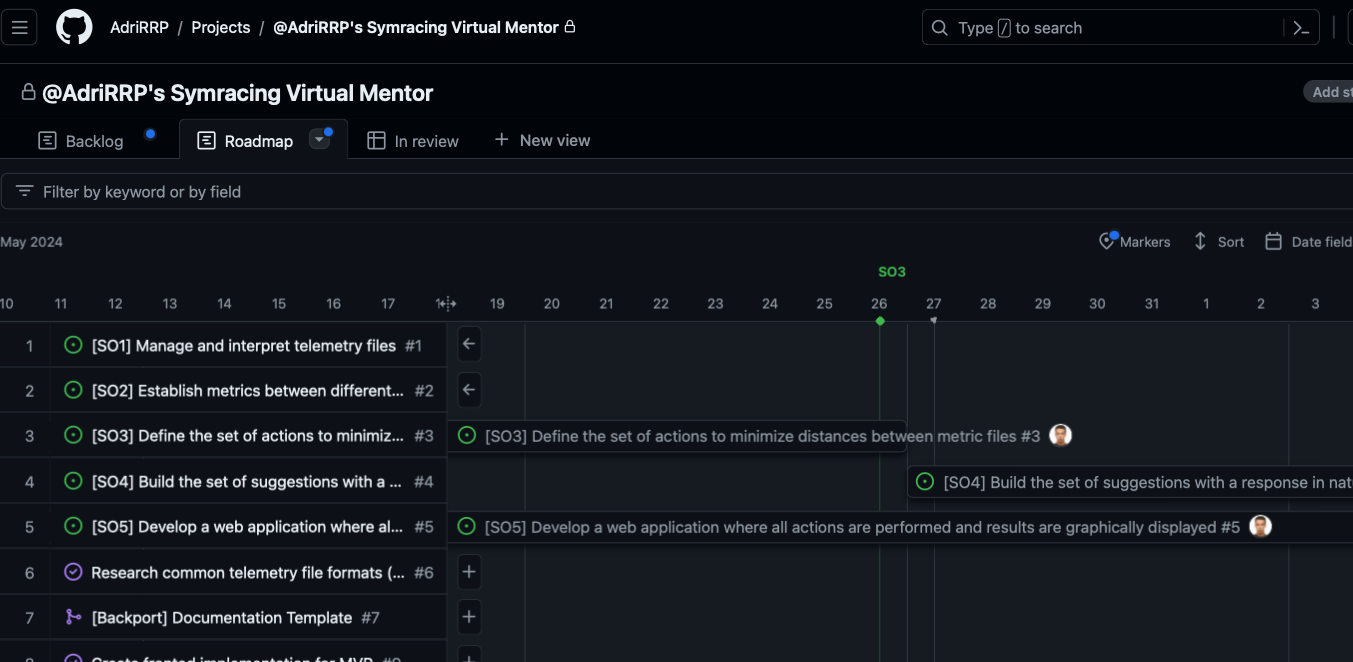
\includegraphics[width=0.8\linewidth]{./figs/herramientas/desarrollo/ghproject_roadmap.png}
	\caption[Captura de roadmap de GitHub Projects]{Captura de roadmap de GitHub Projects}
 \label{fig:ghp_milestones}
\end{figure}


El uso del tablero de tareas en GitHub Projects ha sido una herramienta fundamental en la gestión ágil de este proyecto, proporcionó una visualización clara y estructurada del flujo de trabajo además de facilitar la colaboración y el seguimiento del progreso. El tablero de GitHub Projects se organizó en cinco paneles distintos: ''milestones'' (hitos), ''backlog'' (lista de tareas pendientes), ''in progress'' (en curso), ''ready'' (listas para ser ejecutadas) y ''done'' (finalizadas) (\autoref{fig:ghp_board}).

\begin{figure}[H]
	\centering
	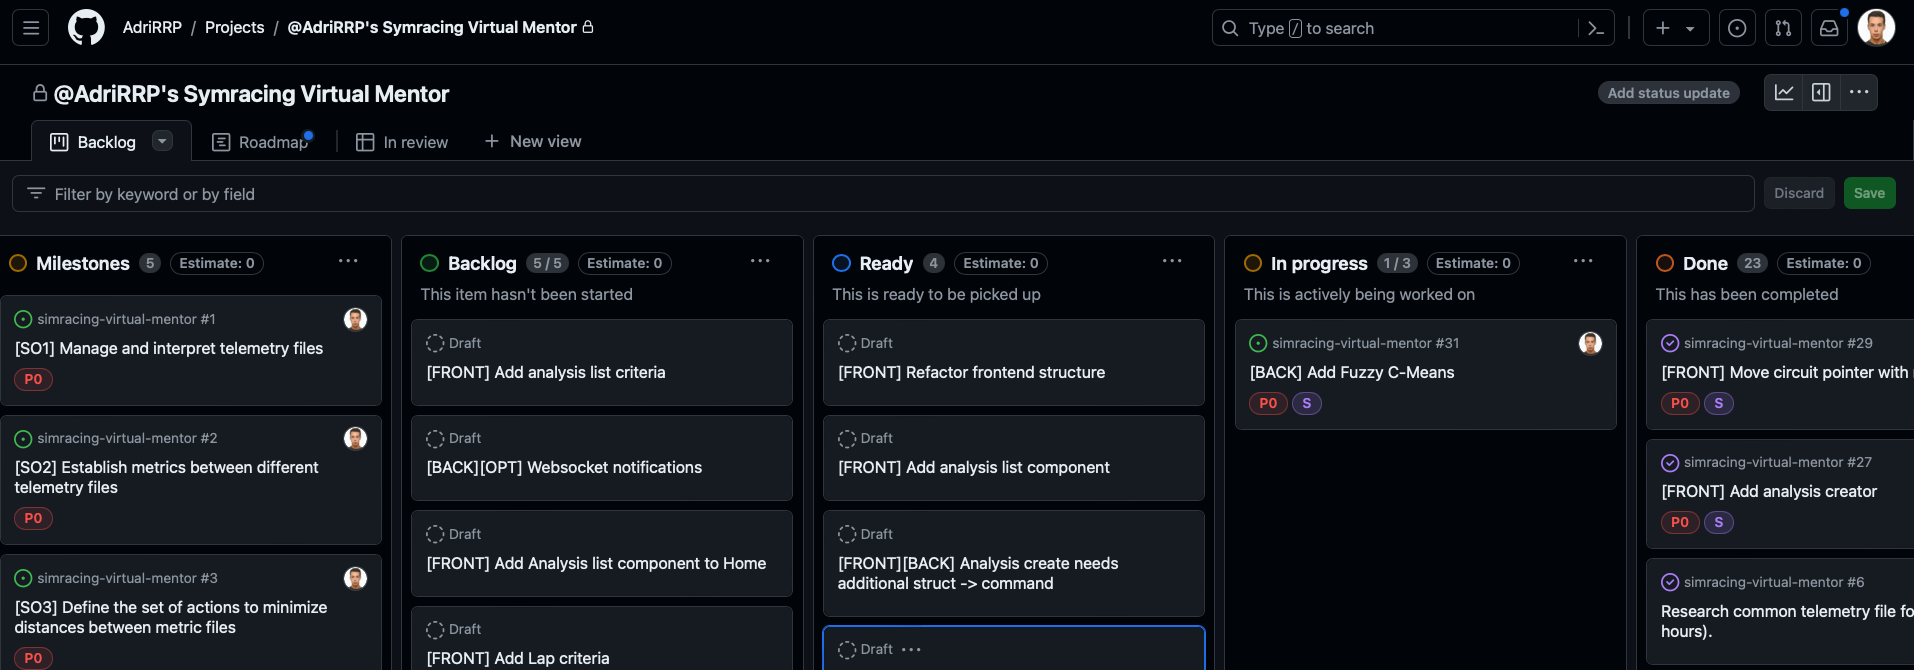
\includegraphics[width=0.9\linewidth]{./figs/herramientas/desarrollo/ghproject_board.png}
	\caption[Captura de tablero de GitHub Projects]{Captura de tablero de GitHub Projects}
    \label{fig:ghp_board}
\end{figure}

\begin{itemize}[noitemsep]
\item El panel \textbf{''milestones''} permitió a los miembros del equipo visualizar el progreso de los hitos de un vistazo, asegurando que los objetivos a largo plazo se  mantenían en el horizonte y se alineaban con las expectativas del cliente.
\item El panel \textbf{''backlog''} contenía todas las tareas necesarias para completar los hitos, proporcionando un depósito centralizado de trabajo pendiente que se gestionó y priorizó continuamente.
\item El panel \textbf{''ready''} indicaba qué tareas estaban listas para ser abordadas tras haber pasado por el proceso de refinamiento y priorización.
\item El panel \textbf{''in progress''} mostraba las tareas que estaban desarrollándose, permitiendo al equipo y a los interesados ver qué trabajo se estaba llevando a cabo en tiempo real.
\item El panel \textbf{''done''} contenía las tareas completadas, ofreciendo una visión clara de lo que ya se había logrado y ayudando a medir el progreso de los objetivos establecidos.\\
\end{itemize}

Desde GitHub Projects también se gestionaron las incidencias. Cada incidencia se daba de alta con un título y una descripción, además se le asignaba un estado inicial de borrador (draft). Durante las reuniones de planificación del sprint, en las que se revisaba el progreso y se establecían nuevos objetivos con el cliente, se examinaban estas incidencias o se creaban nuevas. Se les asignaba una prioridad (etiquetadas como P0, P1 o P2) para indicar su urgencia. Además, cada incidencia recibía una talla, un concepto similar a los puntos de esfuerzo de Scrum que cuantifica el esfuerzo requerido, utilizando una escala similar a los tamaños de ropa, que va desde XS hasta XL (\autoref{fig:ghp_issue}). Posteriormente, la incidencia se movía al backlog para que el programador pudiera asignársela.

\begin{figure}[H]
	\centering
	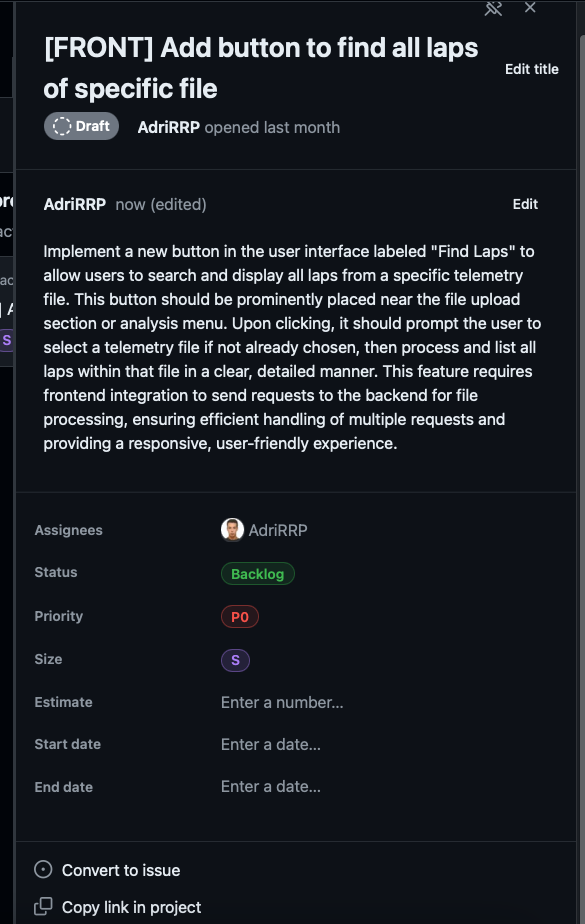
\includegraphics[width=0.30\linewidth]{./figs/herramientas/desarrollo/ghproject_issue.png}
	\caption[Captura de incidencia de GitHub Projects]{Captura de incidencia de GitHub Projects}
    \label{fig:ghp_issue}
\end{figure}

\subsection{Domain Driven Design \textit{(\ac{ddd}}) y Arquitectura Hexagonal}
La adopción de \ac{ddd} y la Arquitectura Hexagonal en este proyecto fue una decisión estratégica que permitió manejar la complejidad y asegurar la flexibilidad y escalabilidad del entrenador virtual de Simracing.

\begin{itemize}[noitemsep]
\item \textbf{Domain-Driven Design}: \ac{ddd} se centra en construir un modelo de dominio que refleje con precisión los conceptos y reglas del dominio específico del negocio. En este proyecto, se ha aplicado \ac{ddd} para estructurar las capas de dominio y aplicación de manera efectiva, asegurando que la lógica de negocio esté bien definida y separada de las preocupaciones técnicas. Esto permite una mejor alineación con los requisitos del cliente y facilita la colaboración entre desarrolladores y expertos en el dominio \cite{Evans2004}. La estructura de directorios del proyecto refleja esta separación, con módulos claramente definidos para diferentes partes del dominio, como \textit{ibt\_extractor, analysis, file y lap}.
\item \textbf{Arquitectura Hexagonal}: La Arquitectura Hexagonal, propuesta por Alistair Cockburn, busca desacoplar el núcleo de la aplicación de las interfaces externas (\autoref{fig:hex_arch}), permitiendo que el sistema sea más adaptable a cambios futuros y facilitando la integración con nuevas tecnologías \cite{Cockburn2005}. En este proyecto, la arquitectura hexagonal se ha implementado mediante la separación de los componentes de la aplicación en capas bien definidas, con directorios dedicados a infraestructura, aplicación, y dominio. Esto no sólo ha mejorado la mantenibilidad del código, sino que también ha permitido realizar pruebas más efectivas y gestionar la complejidad de manera más eficiente.
\end{itemize}

\begin{figure}[H]
	\centering
	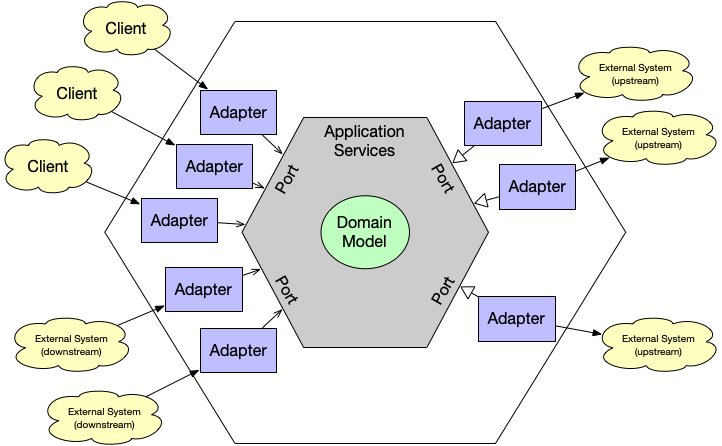
\includegraphics[width=0.5\linewidth]{./figs/herramientas/desarrollo/hexagonal.png}
	\caption[Esquema de Arquitectura Hexagonal]{Esquema de Arquitectura Hexagonal \cite{hexagonal_architecture}}
    \label{fig:hex_arch}
\end{figure}

La combinación de \ac{ddd} y la Arquitectura Hexagonal en este proyecto ha permitido desarrollar un sistema modular y escalable, con un backend robusto basado en principios de diseño estratégico y táctico. El uso de eventos y suscriptores en el backend, junto con la implementación de controladores y repositorios, ha asegurado que la lógica de negocio esté desacoplada de las interfaces técnicas, facilitando la evolución del sistema según las necesidades de los clientes.

\section{Recursos}
En esta sección se detallan los recursos que han sido necesarios para la realización del proyecto, clasificados en hardware, software y humanos, éstos últimos revisados en la sección \hyperref[sec:impl_xp]{metodología de desarrollo}. Además, se incluye una estimación del coste total del proyecto basada en estos recursos. Este análisis ha permitido una comprensión clara de las inversiones requeridas y de cómo se han distribuido los esfuerzos, así como las herramientas empleadas para el desarrollo del asistente virtual de Simracing.

\subsection{Recursos Hardware}
En esta sección se describen los recursos hardware utilizados durante  el desarrollo del proyecto. Este análisis incluye tanto los componentes principales del hardware como sus características relevantes.

\begin{itemize}
\item MacBook Pro M2 (Apple M2 Pro, 16GB RAM, 1TB SSD, monitor Liquid Retina XDR 14 pulgadas).
\item 2 Monitores Phillips Brilliance 241B (24 pulgadas, Full HD).
\item Ratón MSI Interceptor DS300 (7.200 DPI, ergonómico).
\item Teclado Razer Huntsman (mecánico, retroiluminado).
\item Estación de anclado StarTech DK30A2DHU (USB-C, dual HDMI).
\item Router TP-Link Archer AX50.
\end{itemize}

\begin{figure}[H]
	\centering
	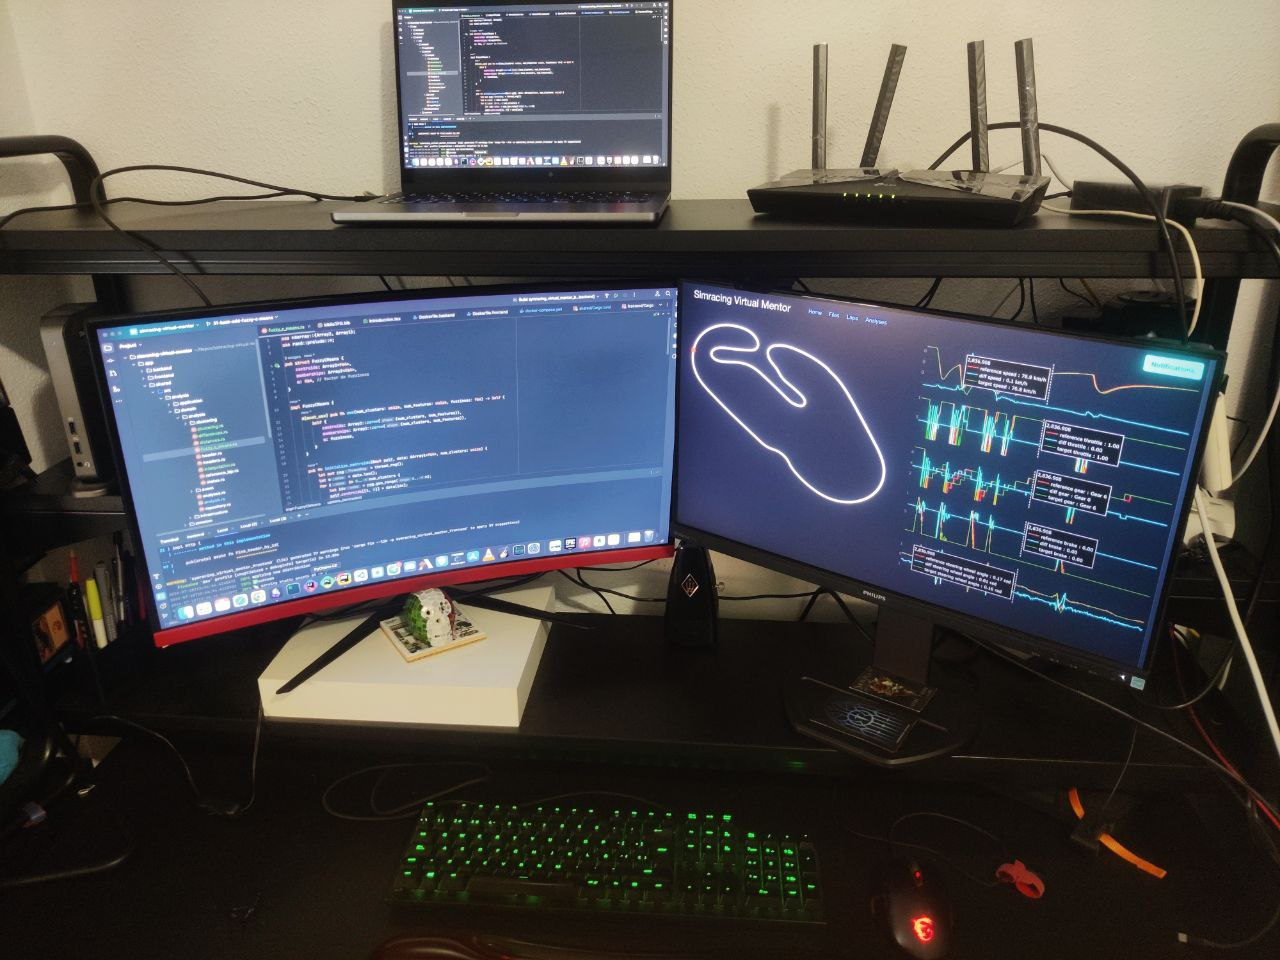
\includegraphics[width=0.70\linewidth]{./figs/herramientas/hardware/recursos_hardware.png}
	\caption[Recursos Hardware utilizados]{Recursos Hardware utilizados}
    \label{fig:recursos_hardware}
\end{figure}


\subsection{Recursos Software}
\subsubsection*{Sistemas Operativos}
\begin{itemize}
\item macOS Sonoma 14.5 (23F79) \cite{macos14_5_release_notes}
\end{itemize}

\subsubsection*{Lenguajes}
\begin{itemize}
\item Programación
    \begin{itemize}
    \item \textbf{Rust 1.79.0}: Lenguaje de programación que enfatiza seguridad, concurrencia y eficiencia, ideal para desarrollar aplicaciones de alto rendimiento sin comprometer la robustez \cite{rust_release_notes_1_79}.
    \end{itemize}
\item Scripting
    \begin{itemize}
    \item \textbf{JavaScript}: Lenguaje de programación interpretado que se utiliza para el desarrollo de aplicaciones web dinámicas y la manipulación del \ac{dom} \cite{mozilla_js}.
    \item \textbf{Dockerfile Syntax}: Lenguaje de configuración utilizado para definir entornos y aplicaciones Docker mediante instrucciones y comandos específicos en un archivo de texto estructurado \cite{dockerfile}.
    \item \textbf{Bash}: Lenguaje de scripting utilizado en sistemas Unix para automatización de tareas y gestión de comandos \cite{bash}.
    \end{itemize}
\item Marcado
    \begin{itemize}
    \item \textbf{\ac{html}}: Lenguaje de marcado  estándar para crear y estructurar páginas web \cite{html}.
    \item \textbf{\ac{json}}: Formato ligero de intercambio de datos fácil de leer y escribir \cite{json}.
    \item \textbf{\ac{yaml}}: Formato de serialización de datos legible por humanos que se utiliza principalmente para archivos de configuración \cite{yaml}.
    \item \textbf{\ac{toml}}: Lenguaje de marcado diseñado para la configuración, enfocándose en la simplicidad y legibilidad humana \cite{toml}.
    \end{itemize}
\item Estilo
    \begin{itemize}
    \item \textbf{\ac{css}}: Lenguaje de estilo usado para describir la presentación de un documento \ac{html} \cite{rust_release_notes_1_79}.
    \end{itemize}
\end{itemize}
\subsubsection*{Bases de Datos}
\begin{itemize}
\item \textbf{MongoDB 7.0} Base de datos NoSQL orientada a documentos \cite{mongodb}.
\item \textbf{MongoDB Compass 1.43.1}: interfaz gráfica para MongoDB que permite explorar, analizar y manipular los datos \cite{mongodb_compass}.
\end{itemize}

\subsubsection*{Librerías}
\begin{itemize}
\item Rust
    \begin{itemize}
    \item \textbf{async-trait 0.1.80}: Permite definir y utilizar traits asíncronos en Rust \cite{async_trait}.
    \item \textbf{axum 0.7.5}: Framework para construir aplicaciones web en Rust con soporte para Tokio \cite{axum}.
    \item \textbf{base64 0.22.1}: Librería para la codificación y decodificación de datos en Base64 \cite{base64}.
    \item \textbf{bson 2.11.0}: Implementación de BSON para Rust, utilizada para trabajar con MongoDB \cite{bson}.
    \item \textbf{chrono 0.4.38}: Librería para la manipulación y formateo de fechas y tiempos \cite{chrono}.
    \item \textbf{config 0.14.0}: Proporciona soporte para la configuración basada en archivos y entornos \cite{config}.
    \item \textbf{futures 0.3.30}: Librería para la programación asíncrona y manejo de futuros en Rust \cite{futures}.
    \item \textbf{futures-util 0.3.30}: Utilidades adicionales para trabajar con futuros en Rust \cite{futures_util}.
    \item \textbf{gloo 0.11.0}: Conjunto de utilidades para el desarrollo de aplicaciones web en Rust \cite{gloo}.
    \item \textbf{gloo-events 0.1}: Librería para trabajar con eventos en aplicaciones web \cite{gloo_events}.
    \item \textbf{gloo-net 0.5.0}: Librería para realizar solicitudes de red en aplicaciones web \cite{gloo_net}.
    \item \textbf{js-sys 0.3.69}: Enlaza cada \ac{api} del sistema JavaScript con Rust \cite{js_sys}.
    \item \textbf{log 0.4.21}: Proporciona una interfaz de registro de logs para Rust \cite{log}.
    \item \textbf{mime 0.3.17}: Librería para trabajar con tipos MIME \cite{mime}.
    \item \textbf{mockall 0.12.1}: Herramienta para crear mocks en Rust durante las pruebas \cite{mockall}.
    \item \textbf{mongodb 2.8.2}: Cliente oficial de MongoDB para Rust \cite{mongodb_crate}.
    \item \textbf{ndarray 0.15.6}: Librería para el manejo de arreglos multidimensionales en Rust \cite{ndarray}.
    \item \textbf{plotly 0.8.4}: Librería para crear gráficos interactivos en Rust \cite{plotly}.
    \item \textbf{rand 0.8.5}: Librería para la generación de números aleatorios \cite{rand}.
    \item \textbf{reqwest 0.12.4}: Cliente \ac{http} simple y eficaz para Rust \cite{reqwest}.
    \item \textbf{serde 1.0.203}: Librería de serialización y deserialización en Rust \cite{serde}.
    \item \textbf{serde-json 1.0.117}: Extensión de Serde para trabajar con JSON \cite{serde_json}.
    \item \textbf{serde-wasm-bindgen 0.6.5}: Librería para la serialización y deserialización con wasm-bindgen \cite{serde_wasm_bindgen}.
    \item \textbf{serde-yaml 0.9}: Extensión de Serde para trabajar con YAML \cite{serde_yaml}.
    \item \textbf{sha256 1.5.0}: Librería para calcular hashes SHA-256 \cite{sha256}.
    \item \textbf{thiserror 1.0.61}: Proporciona una manera ergonómica de definir errores \cite{thiserror}.
    \item \textbf{tokio 1.38.0}: Runtime asíncrono para Rust con soporte para I/O y timers \cite{tokio}.
    \item \textbf{tower-http 0.5.2}: Conjunto de utilidades y middleware para trabajar con servicios \ac{http} \cite{tower_http}.
    \item \textbf{tracing 0.1.40}: Librería para instrumentar aplicaciones Rust para el registro de logs estructurados \cite{tracing}.
    \item \textbf{tracing-subscriber 0.3.18}: Colección de suscriptores para manejar la salida de tracing \cite{tracing_subscriber}.
    \item \textbf{urlencoding 2.1.3}: Librería para la codificación y decodificación de URLs \cite{urlencoding}.
    \item \textbf{uuid 1.8.0}: Librería para la generación y manejo de \ac{uuid} \cite{uuid}.
    \item \textbf{wasm-bindgen 0.2.92}: Proporciona soporte para la interoperabilidad entre Rust y WebAssembly \cite{wasm_bindgen}.
    \item \textbf{wasm-bindgen-futures 0.4.42}: Extensión de wasm-bindgen para trabajar con futuros \cite{wasm_bindgen_futures}.
    \item \textbf{wasm-bindgen-file-reader 1.0.0}: Librería para la lectura de archivos en aplicaciones WebAssembly \cite{wasm_bindgen_file_reader}.
    \item \textbf{wasm-logger 0.2.0}: Implementación de un logger para aplicaciones WebAssembly \cite{wasm_logger}.
    \item \textbf{web-sys 0.3.69}: Enlaza las \ac{api}s del sistema Web con Rust \cite{web_sys}.
    \item \textbf{yew 0.21}: Framework para el desarrollo de aplicaciones web con WebAssembly \cite{yew}.
    \item \textbf{yew-hooks 0.3.2}: Conjunto de hooks para el framework Yew \cite{yew_hooks}.
    \item \textbf{yew-router 0.18.0}: Librería para el enrutamiento en aplicaciones Yew \cite{yew_router}.
    \end{itemize}
\item JavaScript
    \begin{itemize}
    \item \textbf{Plotly JS 2.33.0}: Librería de gráficos interactivos \cite{plotly_js}.
    \end{itemize}
\item \ac{css}
    \begin{itemize}
    \item \textbf{Bulma 1.0.0}: Framework \ac{css} moderno y adaptable. 
    \end{itemize}
\end{itemize}

\subsubsection*{Herramientas de construcción}
\begin{itemize}
\item \textbf{Cargo 1.79.0}: Gestor de paquetes Rust \cite{rust_cargo}.
\item \textbf{Trunk 0.20.2}: Herramienta para construir y desplegar aplicaciones Web basadas en WebAssembly para Rust \cite{trunk}.
\item \textbf{xx 1.4.0}: Herramienta de compilación cruzada y multi-plataforma \cite{xx}.
\end{itemize}

\subsubsection*{Herramientas de desarrollo}
\begin{itemize}
\item \textbf{RustRover 2024.1}: Entorno de desarrollo para Rust \cite{rust_rover}.
\item \textbf{Vim 9.0}: Editor de texto avanzado \cite{vim}.
\item \textbf{xxd 1.4.0}: Herramienta para visualizar datos en hexadecimal \cite{xxd}.
\item \textbf{Google Chrome 126.0.6478.127}: Navegador web desarrollado por Google \cite{chrome}.
\end{itemize}

\subsubsection*{Documentación}
\begin{itemize}
\item \textbf{\LaTeX}: Sistema de preparación de documentos que utiliza macros y formato TEX \cite{latex_project}.
\item \textbf{Overleaf}: Plataforma colaborativa para redacción científica en LaTeX \cite{overleaf}.
\item \textbf{ChatGPT 4o}: Modelo de lenguaje desarrollado por OpenAI utilizado para asistir en la redacción, estructuración y documentación del contenido de este proyecto \cite{chatgpt}.
\end{itemize}

\subsection{Coste}
En esta sección se realiza una estimación de los costes totales del proyecto, teniendo en cuenta los recursos hardware y humanos necesarios. El software utilizado es de carácter libre, por lo que no se incluye en la estimación de costes. A continuación se presentan los detalles y cálculos:
\begin{itemize}
    \item \textbf{Costes de recursos humanos:}
    \begin{itemize}
    \item Desarrollador Rust (nivel medio): 200 horas.
    \item Gerentes (clientes/directores del trabajo): 20 horas cada uno.
    \item Consultor experto en Simracing: 8 horas.
    \end{itemize}

    \item Según los datos del mercado laboral en España \cite{randstad,glassdoor,kiwiremoto}:
    \begin{itemize}
    \item Salario medio de un desarrollador Rust nivel medio: 25 €/hora.
    \item Salario medio de un gerente: 35 €/hora.
    \item Salario medio de un consultor: 45 €/hora.
    \end{itemize}

    \item \textbf{Costes de recursos hardware:}
    \begin{itemize}
    \item MacBook Pro M2 Pro de 14 pulgadas: 2.400 €.
    \item 2 Monitores Phillips Brilliance 241B: 400 € (200 € cada uno).
    \item Ratón MSI Interceptor DS300: 50 €.
    \item Teclado Razer Huntsman: 150 €.
    \item Estación de anclado StarTech DK30A2DHU: 200 €.
    \item Router TP-Link Archer AX50: 150 €.
    \end{itemize}

    \item \textbf{Cálculo de costes:}
    \begin{itemize}
    \item Coste del desarrollador: 200 horas * 25 €/hora = 5.000 €.
    \item Coste de los gerentes: 2 * 20 horas * 35 €/hora = 1.400 €.
    \item Coste del consultor: 8 horas * 45 €/hora = 360 €.
    \item Coste total del hardware: 2.400 € + 400 € + 50 € + 150 € + 200 € + 150 € = 3.350 €.
    \end{itemize}
\end{itemize}

\begin{table}[H]
\centering
\begin{tabular}{|l|c|}
\hline
\textbf{Recurso} & \textbf{Coste (€)} \\ \hline
Desarrollador (200 horas a 25 €/hora) & 5.000 \\ \hline
Gerentes (2 personas, 20 horas cada una a 35 €/hora) & 1.400 \\ \hline
Consultor (8 horas a 45 €/hora) & 360 \\ \hline
MacBook Pro M2 Pro de 14 pulgadas & 2.400 \\ \hline
2 Monitores Phillips Brilliance 241B & 400 \\ \hline
Ratón MSI Interceptor DS300 & 50 \\ \hline
Teclado Razer Huntsman & 150 \\ \hline
Estación de anclado StarTech DK30A2DHU & 200 \\ \hline
Router TP-Link Archer AX50 & 150 \\ \hline
Electricidad (uso proporcional: 20\% de 6 meses a 50 €/mes) & 60 \\ \hline
Internet (uso proporcional: 50\% de 6 meses a 30 €/mes) & 90 \\ \hline
\textbf{Total} & \textbf{10.260} \\ \hline
\end{tabular}
\caption{Coste total del proyecto desglosado por recursos}
\label{tab:costes_proyecto}
\end{table}

\section{Aseguramiento de la Calidad}
El aseguramiento de la calidad en este proyecto fue gestionado de manera integral utilizando varias estrategias y herramientas clave. A continuación se describe cómo se aplicaron estas medidas.

\subsection{Pruebas}
Rust ofrece un robusto sistema de testing integrado que se utilizó para realizar las pruebas del entrenador virtual de Simracing.
Se utilizó el enfoque de \ac{ddd} para estructurar el proyecto de manera que la lógica de negocio estuviera bien definida y aislada. Esto facilitó la creación de \textbf{pruebas unitarias} para el dominio de la aplicación.
Las \textbf{pruebas de integración} verificaron la coherencia y el correcto funcionamiento de los diferentes servicios (casos de uso/historias de usuario) sin necesidad de disponer de la infraestructura (repositorios y servicios externos) y por tanto sin acoplarse a ella. Esto fue posible gracias a \ac{ddd} y la separación entre las capas de aplicación e infraestructura.


\subsection{Análisis y Formato de Código}
Para mantener un formato de código estándar y mejorar la calidad del mismo, se utilizaron las herramientas \textbf{Cargo fmt} y \textbf{Clippy}. Cargo fmt aseguró que todo el código siguiera las convenciones de estilo de Rust, mejorando la legibilidad y facilitando la colaboración entre desarrolladores. Clippy se utilizó para realizar análisis estáticos del código, identificando posibles errores, malas prácticas y sugiriendo mejoras.


\subsection{Flujo de \ac{cicd} con GitHub Actions}
Se estableció un flujo de integración y entrega continua \ac{cicd} utilizando GitHub Actions \cite{github_actions}. Este flujo automatizado aseguraba que todos las pruebas se ejecutaran antes de integrar cambios en la rama principal (main). El proceso de \ac{cicd} incluía controles de calidad que utilizaban Codecov \cite{codecov} para medir la cobertura de los tests y garantizar que se mantenían altos estándares de calidad.

Los tres archivos clave en la carpeta `.github/workflows` fueron:
\begin{itemize}
    \item \textbf{clippy.yaml}: Configuración para ejecutar clippy y asegurar que el código seguía las mejores prácticas.
    \item \textbf{coverage.yaml}: Configuración para medir la cobertura de los tests con Codecov.
    \item \textbf{tests.yaml}: Configuración para ejecutar todos los tests unitarios e integrados del proyecto.
\end{itemize}

Estas prácticas permitieron identificar y corregir errores de manera temprana y aseguraron que el código cumpliera consistentemente con los estándares de calidad definidos. El uso de estas herramientas y metodologías no sólo mejoró la calidad del software, sino que también facilitó un desarrollo más ágil y eficiente.

\section{Riesgos}
Al inicio del proyecto de desarrollo del entrenador virtual para Simracing, se identificaron y evaluaron varios riesgos potenciales que podrían afectar el éxito del mismo. Estos riesgos se abordaron con un enfoque sistemático para mitigar su impacto y garantizar un desarrollo fluido.

\begin{itemize}
    \item Uno de los riesgos principales identificados fue la \textbf{complejidad técnica del proyecto}. La implementación de \ac{ddd} y la Arquitectura hexagonal implicaba un nivel elevado de abstracción y modularidad que requería una comprensión profunda de estos conceptos por parte del desarrollador. Esto se mitigó mediante el estudio y la aplicación gradual de estas metodologías, así como con la consultoría especializada de un experto en Simracing.
    \item Otro riesgo significativo fue la \textbf{integración de tecnologías y herramientas diversas}. La utilización de Rust como lenguaje principal, junto con MongoDB para la gestión de datos, y herramientas como GitHub Actions para \ac{cicd}, requería una integración cuidadosa y coordinada. Para mitigar este riesgo, se definieron claramente las responsabilidades de cada componente del sistema y se implementaron pruebas unitarias e integradas para asegurar la correcta interoperabilidad.
    \item Además, la \textbf{gestión de la calidad del código} se identificó como un riesgo crucial. La utilización de Clippy y Cargo fmt fue esencial para mantener un estándar de codificación elevado y consistente. Sin embargo, se reconoció que la configuración de estas herramientas podría ser desafiante y consumir tiempo. Este riesgo se manejó configurando Clippy con sus vertientes más restrictivas desde el inicio y asegurando que el desarrollador se familiarizara con su uso.
    \item Finalmente, el riesgo asociado al \textbf{despliegue y mantenimiento del sistema} se abordó mediante la implementación de un flujo de \ac{cicd} robusto utilizando GitHub Actions y Codecov. Este enfoque permitió una integración continua y un despliegue controlado, minimizando los errores y asegurando una cobertura de pruebas adecuada antes de cualquier fusión en la rama principal del proyecto.
\end{itemize}

En resumen, la identificación y gestión proactiva de estos riesgos fue fundamental para el éxito del proyecto, permitiendo abordar desafíos técnicos complejos y asegurar un alto nivel de calidad en el desarrollo del entrenador virtual para Simracing.
\chapter{Desarrollo}
\label{cap:Desarrollo}

En esta sección se describirá las diferentes fases del ciclo de desarrollo de software de acuerdo al plan de gestión expuesto en el capítulo \ref{cap:Planificacion}. 

\section{Requisitos y análisis del sistema}
En este apartado se presentarán los objetivos y el catálogo de requisitos del proyecto: funcionales, no funcionales, de información, reglas de negocio, etc.

Una vez catalogados los requisitos del sistema se procederá con su análisis empleando el lenguaje de modelado UML. El análisis mencionado incluirá:
\begin{itemize}
\item \textbf{Modelo conceptual}. En él se identifican clases, atributos, relacionales, etc.

\item \textbf{Modelo de casos de uso}. Representan las interacciones entre los actores y el sistema bajo estudio.

\item \textbf{Modelo de interfaz de usuario}. Puede consistir en un prototipo de baja fidelidad de la interfaz de usuario.
\end{itemize}

\subsection{Análisis de Formatos de Telemetría en Simuladores de Carreras}
Dentro del análisis del sistema, es crucial comprender los formatos de ficheros de telemetría utilizados por las plataformas de simuladores de carreras. Estos formatos presentan particularidades que afectan la extracción y gestión de datos. A continuación, se detallan algunos aspectos relevantes:

\begin{itemize}
\item \textbf{Formatos Propietarios y Herramientas de Extracción}. La mayoría de los simuladores de carreras utilizan formatos binarios propietarios para sus ficheros de telemetría, cuya especificación no es de dominio público. Esto implica dificultades para acceder y comprender estos datos, ya que se requiere de herramientas específicas para su extracción y análisis.

\item \textbf{Elección de iRacing y su Formato .ibt}. iRacing destaca como una plataforma de sim-racing ampliamente utilizada, lo que ha motivado el desarrollo de herramientas libres para la gestión de sus ficheros de telemetría en formato .ibt. Este formato binario contiene información detallada sobre parámetros como posición en pista, velocidad, aceleración, frenado, entradas del piloto, entre otros.
\item \textbf{Herramientas de Extracción y Análisis}. Dentro de la comunidad de sim-racing, existen diversas herramientas de código abierto que permiten la extracción y análisis de los ficheros .ibt de iRacing. Estas herramientas facilitan la visualización de datos de rendimiento, la comparación de sesiones y la mejora del desempeño en pista.
\end{itemize}

\section{Diseño del sistema}
En esta sección se define la arquitectura lógica general del sistema. Para describirla se puede emplear un modelo como C4~\cite{Brown22}, el cual permite representar la arquitectura de un sistema software mediante varios diagramas a distintos niveles de abstracción.

\section{Implementación del sistema}
En este apartado se describirá la organización del código fuente y \emph{scripts}, describiendo el propósito de los distintos ficheros y su distribución en paquetes y directorios. Puede ser conveniente incluir alguna porción significativa de código fuente que sea de especial relevancia por su funcionalidad.

En el desarrollo de proyectos software cobra especial importancia el empleo de sistemas de control de versiones junto a repositorios en línea. Estas herramientas se convierten en esenciales para disponer de un registro histórico del desarrollo que también puede ayudar a evaluar el trabajo realizado. Por este motivo, en la memoria del proyecto se debe indicar la dirección de los repositorios empleados (p.~ej.,~Github).

\section{Pruebas del sistema}
En esta sección se describirá el plan de pruebas del sistema incluyendo todos los tipos llevados a cabo. El desarrollo de la sección debería tratar los aspectos siguientes:
\begin{itemize}[noitemsep]
\item \textbf{Estrategia}. Donde se indica el alcance de las pruebas y los procedimientos.

\item \textbf{Pruebas unitarias}. Destinadas a localizar errores en cada nuevo módulo software desarrollado antes de su integración con el resto del sistema.

\item \textbf{Pruebas de integración}. Su objetivo es localizar errores en subsistemas completos analizando la interacción entre varios módulos de software.

\item \textbf{Pruebas de sistema}. Contempla las pruebas funcionales con las que se realiza el análisis del buen funcionamiento de la implementación de los casos de uso del sistema. Además, en estas pruebas se comprueba el funcionamiento respecto a los requisitos no funcionales: eficiencia, seguridad, etc.

\item \textbf{Pruebas de aceptación}. Su intención es demostrar, con la participación del cliente, que el producto está listo para su puesta en funcionamiento en el entorno producción.
\end{itemize}

\section{Despliegue}
Esta sección recoge la arquitectura física propuesta del sistema, las instrucciones para su despliegue, operación y mantenimiento del
nivel de servicio.

Es muy importante que todas las justificaciones aportadas se sustenten no solo en juicios de valor sino en evidencias tangibles como: historiales de actividad, repositorios de código y documentación, porciones de código, trazas de ejecución, capturas de pantalla, demos, etc.

\chapter{Conclusiones}
\label{cap:Conclusiones}

En este capítulo se presentan las conclusiones del trabajo realizado, evaluando el grado de cumplimiento de los objetivos planteados y destacando las competencias adquiridas a lo largo del desarrollo del proyecto. Asimismo, se discutirán los trabajos derivados y futuros que pueden surgir a partir de este proyecto y se ofrecerá una valoración personal sobre las lecciones aprendidas y la experiencia obtenida.


\section{Objetivos alcanzados}

El objetivo principal del \ac{tfg} era diseñar y desarrollar un entrenador virtual de código abierto capaz de interpretar archivos de telemetría del software iRacing. Este entrenador debía proporcionar un análisis detallado, permitiendo la visualización de métricas comparativas entre dos vueltas en un circuito, y ofrecer recomendaciones de mejora de la conducción en lenguaje natural. Este objetivo se ha cumplido satisfactoriamente, desarrollando una herramienta robusta y eficiente que facilita la comprensión y aplicación de las mejoras por parte de los pilotos, contribuyendo a su rendimiento y desarrollo en el Simracing.

Para alcanzar este objetivo general, se plantearon los siguientes objetivos específicos, todos los cuales han sido alcanzados:

\subsection{Adquirir y procesar datos de telemetría}
\begin{itemize}
    \item Se investigó cómo se adquieren y transfieren los ficheros de telemetría .ibt de iRacing y se consiguió una muestra.
    \item Se estudió el formato de telemetría .ibt de iRacing.
    \item Se desarrolló un módulo para la lectura y decodificación de archivos de telemetría en formato .ibt.
\end{itemize}

\subsection{Fijar las métricas de comparación}
\begin{itemize}
    \item Se identificaron y seleccionaron las variables de telemetría relevantes para su posterior comparación.
    \item Se desarrolló un modelo que define y permite comparar los datos de telemetría.
\end{itemize}

\subsection{Comparar datos de telemetría y aplicar aprendizaje no supervisado para clasificar diferencias}
\begin{itemize}
    \item Se implementaron métodos para la comparación de datos de telemetría.
    \item Se aplicaron técnicas de aprendizaje no supervisado para clasificar las diferencias observadas.
\end{itemize}

\subsection{Construir el conjunto de sugerencias con una respuesta en lenguaje natural}
\begin{itemize}
    \item Se desarrolló un método sistemático para la asignación de etiquetas interpretables a las diferencias en los datos de telemetría.
    \item Se creó un sistema de generación de sugerencias en lenguaje natural basado en la interpretación de las diferencias.
    \item Se diseñó una interfaz que presenta las sugerencias de manera clara y comprensible para el usuario.
\end{itemize}

\subsection{Desarrollar una aplicación web donde se realicen todas las acciones y se muestren gráficamente los resultados}
\begin{itemize}
    \item Se investigaron y evaluaron lenguajes y frameworks adecuados para el desarrollo de aplicaciones web con gráficos interactivos y algoritmos complejos.
    \item Se analizaron los requisitos de rendimiento y escalabilidad necesarios para gestionar eficientemente grandes volúmenes de datos.
    \item Se diseñó una arquitectura que soporta la escalabilidad y la modularidad para facilitar el desarrollo y mantenimiento.
    \item Se exploraron opciones de bases de datos que proporcionan simplicidad y flexibilidad en los cambios de esquema.
    \item Se desarrolló una interfaz de usuario intuitiva y eficiente que permite la visualización gráfica de los resultados.
    \item Se aseguró que la aplicación sea extensible y adaptable para futuras mejoras y colaboraciones en la comunidad de código abierto.
\end{itemize}




\section{Justificación de competencias adquiridas}
En el \ac{tfg} se han aplicado las competencias correspondientes a la Tecnología Específica de Computación:

\begin{description}
\item[CM1:] \emph{Capacidad para tener un conocimiento profundo de los principios fundamentales y modelos de la computación y saberlos aplicar para interpretar, seleccionar, valorar, modelar, y crear nuevos conceptos, teorías, usos y desarrollos tecnológicos relacionados con la informática.} Esta competencia se aplicó en el desarrollo del módulo de lectura y decodificación de archivos de telemetría en formato .ibt, así como en la implementación del algoritmo \ac{fcm} para el análisis de diferencias. Se requirió un conocimiento detallado de los principios fundamentales de la computación para interpretar y modelar los datos de telemetría de iRacing, seleccionar las técnicas de análisis más adecuadas y desarrollar conceptos novedosos para la generación de sugerencias en lenguaje natural.

\item[CM2:] \emph{Capacidad para conocer los fundamentos teóricos de los lenguajes de programación y las técnicas de procesamiento léxico, sintáctico y semántico asociadas, y saber aplicarlas para la creación, diseño y procesamiento de lenguajes.} La implementación del entrenador virtual involucró el uso de Rust, un lenguaje de programación moderno que ofrece seguridad y concurrencia. Se aplicaron conocimientos sobre los fundamentos teóricos del lenguaje y técnicas de procesamiento para desarrollar módulos eficientes y seguros, garantizando un rendimiento óptimo del sistema.

\item[CM3:] \emph{Capacidad para evaluar la complejidad computacional de un problema, conocer estrategias algorítmicas que puedan conducir a su resolución y recomendar, desarrollar e implementar aquella que garantice el mejor rendimiento de acuerdo con los requisitos establecidos.} Se evaluaron diversas estrategias algorítmicas para la clasificación de diferencias y se implementó la que garantizaba el mejor rendimiento. La complejidad computacional del algoritmo \ac{fcm} y la interpolación de datos fueron analizadas para asegurar que el sistema pudiera manejar grandes volúmenes de datos de telemetría de manera eficiente.

\item[CM4:] \emph{Capacidad para conocer los fundamentos, paradigmas y técnicas propias de los sistemas inteligentes y analizar, diseñar y construir sistemas, servicios y aplicaciones informáticas que utilicen dichas técnicas en cualquier ámbito de aplicación.} Esta competencia se reflejó en la aplicación de técnicas de aprendizaje no supervisado, específicamente el algoritmo \ac{fcm}, para clasificar las diferencias en los datos de telemetría y generar recomendaciones inteligentes en lenguaje natural.

\item[CM5:] \emph{Capacidad para adquirir, obtener, formalizar y representar el conocimiento humano en una forma computable para la resolución de problemas mediante un sistema informático en cualquier ámbito de aplicación, particularmente los relacionados con aspectos de computación, percepción y actuación en ambientes o entornos inteligentes.} Se desarrolló un método sistemático para la asignación de etiquetas interpretables a las diferencias en los datos de telemetría, representando el conocimiento humano de manera computable para proporcionar sugerencias de mejora a los pilotos.

\item[CM6:] \emph{Capacidad para desarrollar y evaluar sistemas interactivos y de presentación de información compleja y su aplicación a la resolución de problemas de diseño de interacción persona-computadora.} Se diseñó una interfaz de usuario intuitiva y eficiente que permite la visualización gráfica de los resultados, facilitando la interpretación y toma de decisiones basadas en los datos de telemetría. Se implementaron gráficos interactivos y un cuadro de mandos para presentar la información de manera clara y comprensible.

\item[CM7:] \emph{Capacidad para conocer y desarrollar técnicas de aprendizaje computacional y diseñar e implementar aplicaciones y sistemas que las utilicen, incluyendo las dedicadas a extracción automática de información y conocimiento a partir de grandes volúmenes de datos.} Esta competencia se aplicó en la implementación de técnicas de aprendizaje no supervisado para la clasificación de diferencias y la generación de recomendaciones en lenguaje natural. Se desarrolló un sistema que automatiza la extracción de información y proporciona análisis detallados de los datos de telemetría.
\end{description}

\section{Trabajos derivados y futuros}
Este proyecto ha sentado las bases para futuros trabajos y mejoras. Gracias a su naturaleza de software libre, se pretende que esta herramienta crezca con la colaboración de interesados y la comunidad de usuarios. A continuación, se detallan algunas de las direcciones futuras para el desarrollo y expansión del proyecto:

\begin{itemize}
    \item \textbf{Extensibilidad y colaboración comunitaria:} Las librerías desarrolladas están diseñadas para ser extensibles, permitiendo a otros desarrolladores añadir nuevas funcionalidades y mejorar las existentes. Se planea promocionar el proyecto en foros específicos de Simracing y desarrollo de software libre, invitando a la comunidad a contribuir con sus ideas y mejoras.
    
    \item \textbf{Mejora de la calidad del código:} Se trabajará en la mejora continua de la calidad del código existente, añadiendo más tests unitarios y de integración, así como implementando procesos automáticos de mejora de la calidad. Esto incluye la integración de herramientas de análisis estático y dinámico, y la adopción de prácticas de desarrollo continuo para asegurar la estabilidad y robustez del sistema.
    
    \item \textbf{Análisis online:} Una de las futuras mejoras será la implementación de capacidades de análisis en tiempo real, permitiendo a los usuarios obtener información y recomendaciones durante sus sesiones de entrenamiento. Esto implicará la integración de tecnologías de transmisión en tiempo real y la optimización del procesamiento de datos para minimizar la latencia.
    
    \item \textbf{Configuración del entrenamiento del algoritmo \ac{fcm}:} Se pretende habilitar una interfaz que permita a los usuarios establecer la configuración del entrenamiento del algoritmo \ac{fcm}. Esto ofrecerá mayor flexibilidad y control sobre el proceso de análisis, permitiendo ajustes personalizados que se adapten a las necesidades específicas de cada usuario.
\end{itemize}

Estos trabajos futuros tienen como objetivo no sólo mejorar la funcionalidad y la usabilidad de la herramienta, sino también fomentar una comunidad activa y colaborativa que contribuya al desarrollo continuo del proyecto. La visión a largo plazo es que esta plataforma se convierta en un referente en el ámbito del análisis de telemetría para Simracing, aprovechando las ventajas del software libre y la inteligencia colectiva de sus usuarios y desarrolladores.

\section{Valoración personal}

La realización de este trabajo me ha permitido experimentar de primera mano las aplicaciones prácticas de los conjuntos difusos, trascendiendo su carácter meramente teórico y apreciando su utilidad en problemas reales como el análisis de telemetría en el Simracing. Esta experiencia ha sido enormemente enriquecedora, ya que me ha permitido aplicar conceptos matemáticos avanzados a situaciones concretas, mejorando mi comprensión y habilidades en esta área.

Además, este proyecto me ha brindado la oportunidad de aprender y trabajar con tecnologías muy interesantes y avanzadas, como Rust y su ecosistema. La elección de Rust como lenguaje de programación principal no sólo ha demostrado ser acertada por su eficiencia y seguridad, sino que también ha ampliado significativamente mis conocimientos en programación de sistemas y en el desarrollo de aplicaciones de alto rendimiento.

Uno de los aspectos a mejorar que he identificado a lo largo del proyecto es la sub-estimación del tiempo necesario para la documentación. A menudo, la documentación adecuada es crucial para el éxito y la mantenibilidad de un proyecto, y he aprendido que debe ser tratada con la misma importancia que el desarrollo del código.

En cuanto al tiempo dedicado al proyecto, aunque no ha sido desmesurado, ha sido un desafío significativo equilibrar este trabajo con mis responsabilidades laborales de 8 horas diarias. A pesar de estas dificultades, he logrado dedicar el esfuerzo necesario para completar el proyecto, lo que me ha permitido desarrollar habilidades de gestión del tiempo y organización, esenciales para la realización de proyectos complejos.

En resumen, este proyecto no sólo me ha permitido aplicar y profundizar en conocimientos técnicos avanzados, sino que también ha sido una valiosa experiencia de aprendizaje y crecimiento personal.









%--- (FIN MAINMATTER)


% -------------------------
% No olvides retornar al interlineado sencillo en el resto del documento.
\singlespacing
% -------------------------
% -------------------------
% -------------------------
% -------------------------
%
%--- BACKMATTER
%BEGIN_FOLD
% \backmatter 
% Comentado para que apéndices aparezcan numerados después de la bibliografía


% -------------------------
% --- BIBLIOGRAFÍA
% -------------------------
\cleardoublepage % Necesario para ajustar el avance de página
\phantomsection  % Ojo necesario con hyperref.
\addcontentsline{toc}{chapter}{\bibname} % Añade la bibliografía al Índice de contenidos

% Descomentar si se incluye lista \bibitem desde fichero "refs.bbl"
\newif\ifbibitemrefs\bibitemrefsfalse
% OPT: Activa bibitems para la bibliografía descomentabdi línea sig.
%\bibitemrefstrue 
\ifbibitemrefs  % Se incluye bibitem list desde refs.bbl
	\input{refs.bbl} % OJO: Fichero refs.bbl debe existir
\else % OPT: Estilo en bibliografía
	\bibliography{biblioTFG}   % Nombre del fichero .bib (sin extensión)
	\bibliographystyle{plain}  % Estilo empleado en la bibliografía
\fi
% Estilos nativos incluidos con LaTeX (plain, abbrv, alpha, unsrt).
%
% plain: las referencias se numeran y en la bibliografía las entradas
%        aparecen en orden alfabético.
% abbrv: igual que el anterior pero en la bibliografía los nombres se
%        escriben sólo con la inicial.
%        y el año de publicación. En la bibliografía los nombres 
%        igual que en plain. 
%        .
% unsrt: la bibliografía no aparece por orden alfabético sino por 
%        orden de cita en el texto.
%
%---     Estilos incluidos con BibTeX “no nativos”, pero populares” 
%        para ingenierías (no requieren paquetes adicionales).
% acm:   Numérica con los nombre de autores en mayúsculas y 
%        referencias con ordenación alfabética.
% ieeetr:Para los IEEE Transactions, con citación numérica 
%        y ordenación de referencias por orden de cita.
%========
% apacite: No numérica, con referencias ordenadas alfabéticamente
%          por apellido de autor (requiere paquete 'apacite'). 
%
% NOTA: Cita natbib con estilo apacite
%          La citación mediante este paquete permite el empleo 
%          de comandos del paquete natbib como:
%
%   \citet{key} 				==>> Jones y col. (1990)
%   \citet*{key} 				==>> Jones, Baker, y Smith (1990)
%   \citep{key} 				==>> (Jones y col., 1990)
%   \citep*{key} 				==>> (Jones, Baker, y Smith, 1990)
%   \citep[cap. 2]{key} 		==>> (Jones y col., 1990, cap. 2)
%   \citep[ver][]{key} 			==>> (ver Jones y col., 1990)
%   \citep[ver][pág. 32]{key} 	==>> (ver Jones y col., pág. 32)
%   \citeauthor{key} 			==>> Jones y col.
%   \citeauthor*{key} 			==>> Jones, Baker, y Smith
%   \citeyear{key} 				==>> 1990
% -------------------------
%--- (FIN BIBLIOGRAFÍA)
% -------------------------



% -------------------------
% - ANEXOS: Comentar si no se desean incluir. [OPT.]
% - Mover si se desea que aparezcan antes de la bibliografía.
% -------------------------
% EDITA: Anexos, ajusta a las necesidades añadiendo o quitando
\appendix
\ifspanish
	\part*{\sffamily ANEXOS}
\else
	\part*{\sffamily APPENDICES}
\fi
% Tras este punto los capítulos se numeran con letras.
% Aquí todos los apéndices necesarios
\chapter{Sobre la Bibliografía}
\label{cap:AnexoA}

En los anexos se incluirá, de modo opcional, material suplementario que podrá consistir en manuales de usuario, listados seleccionados de código fuente, esquemas, planos y en general aquel contenido que complementa a la memoria. Se recomienda que no sean excesivamente voluminosos, aunque su extensión no está sometida a la regulación por normativa, ya que esta afecta únicamente al texto principal de la memoria.

En esta plantilla hemos decidido incluir dos anexos. En el primero de ellos se hacen algunos comentarios adicionales sobre la bibliografía. En el segundo se aporta una breve introducción a \LaTeX{} cuya información puede servir de ejemplo de inclusión de ciertos elementos en la preparación de la memoria del TFG.

Todo el material de terceros se debe citar convenientemente sin contravenir los términos de las licencias de uso y distribución de dicho material. Esto se extiende al uso de diagramas y fotografías. El incumplimiento de la legislación vigente en materia de protección de la propiedad intelectual es responsabilidad exclusiva del autor, independientemente de la cesión de derechos que este haya convenido.

La sección de \emph{Bibliografía}, que si se prefiere se puede titular \emph{Referencias}, incluirá un listado ordenado preferentemente por orden alfabético (primer apellido del autor principal), con todas las obras citadas en el texto. En la lista de referencias se especificará para cada obra: autores, título, editorial y año de publicación. Este formato se conseguirá en \LaTeX{} mediante el uso del estilo estándar \texttt{plain} o cualquier otro derivado con estilo de citación numérica. En algunas titulaciones se obliga a una ordenación por orden de cita en el texto que con Bib\TeX{} se puede obtener mediante los estilos estándar \texttt{ieeetr} (estilo para los IEEE \emph{transactions}) y \texttt{unsrt} (estilo \emph{unsorted}). 

Es muy importante tener presente que en esta sección solo se debe incluir las referencias bibliográficas citadas expresamente en el documento. Si se desea incluir fuentes consultadas, pero no citadas, se puede confeccionar con ellas una sección denominada \emph{Material de consulta}, aunque estas referencias se pueden incluir opcionalmente a lo largo del documento como notas a pie de página.

En las titulaciones técnicas se empleará estilo de citación numérico con el número de la referencia entre corchetes. La cita podrá incluir el número de página concreto de la referencia que se desea citar. El uso correcto de la citación implica dejar claro al lector cuál es el texto, material o idea citado. Las obras referenciadas sin mención explícita o implícita al material concreto citado se deberían considerar material de consulta y, por tanto, ser agrupadas como \emph{Material de consulta}, distinguiéndolas claramente de aquellas otras en las que sí se recurre a la citación.

En las titulaciones que requieren un estilo de citación de tipo autor-año (no numérico), se puede incluir el paquete \LaTeX{} \texttt{apacite} (con la opción \texttt{natbibapa}) y especificar este mismo estilo en la sección de bibliografía en el argumento del comando \texttt{bibliographystyle}.

Cuando se desee incluir referencias a páginas genéricas de la Web sin mención expresa a un artículo con título y autor definido, dichas referencias se pueden incluir como notas al pie de página o como un apartado de fuentes de consulta dedicado a \emph{Direcciones de Internet}. Por el contrario, los documentos electrónicos publicados en Internet se pueden incluir empleando el tipo de entrada \texttt{misc} con el comando \texttt{url} como se muestra en la bibliografía que acompaña esta plantilla. Observarás que el campo \texttt{note} se emplea para añadir información adicional como la fecha de la última consulta de fuentes publicadas en Internet, y para la inclusión del DOI de algunas obras para su rápida recuperación. Sin embargo, ten cuidado porque esta estrategia puede necesitar una adaptación con un estilo de citación autor-año.







 % Apéndice A (opcionales)
\chapter{Breve introducción a \LaTeX}
\label{cap:AnexoB}

El contenido del trabajo final de estudios se organiza en capítulos que se subdividen en secciones. Con \LaTeX{} este tipo de organización se realiza de modo inmediato mediante la generación automática de los estilos correspondientes a los títulos de cada sección y su inclusión en la tabla de contenidos. Los ajustes relativos a la generación del formato y estilos asociados a secciones del documento se realizan con el paquete \texttt{titlesec} empleado en esta plantilla.

En las secciones siguientes se comenta la inclusión con \LaTeX{} de distintos elementos de organización de información junto a ejemplos que facilitan su  utilización en la memoria del trabajo.\footnote{Las explicaciones de este anexo forman parte del contenido del curso \href{https://visilab.etsii.uclm.es/?page_id=1468}{<<\LaTeX{} esencial para preparación de TFG y otros documentos académicos>>} de la \href{https://esi.uclm.es/}{ESI-UCLM}.}




\section{Listas}
\label{sec:ejListas}
Existen dos tipos de listas: enumeraciones y listas con viñetas. En el primer tipo los elementos de la lista se preceden de una clave numérica o alfabética, mientras que en el segundo tipo se emplea una viñeta. En ambos casos los elementos se pueden anidar para crear una jerarquía entre ellos. En \LaTeX{} se recomienda la inclusión del paquete \texttt{enumitem} que permite personalizar fácilmente las listas de un documento. A continuación se muestran algunos ejemplos:


\noindent Ejemplo de lista con viñetas personalizadas. 
% Ejemplo: Lista con bullets especiales
% ============
\begin{itemize}
	\item pera
	\item[\ding{43}] manzana % Particularización de viñeta
	\item[\faAward] naranja
\end{itemize}


\noindent Ejemplo de lista condensada con separación mínima, en varias columnas y configuración de la etiqueta.
% Ejemplo: Listas en varias columnas
% ============
\begin{multicols}{2} % El parámetro es el número de columnas de la lista
	\begin{enumerate}[(1),noitemsep]
		\item pera
		\item manzana
		\item naranja
		\item patata
		\item calabaza
		\item fresa
	\end{enumerate}
\end{multicols}


Además del texto, los documentos pueden incluir elementos que enriquecen su contenido facilitando su exposición y comprensión. En las secciones siguientes tratamos brevemente dichos elementos.

\section{Ecuaciones matemáticas}
Para escribir ecuaciones matemáticas con \LaTeX{} se recomienda incluir los paquetes siguientes en el documento: \texttt{amsmath}, \texttt{amsfonts}, \texttt{amssymb}. 

La composición de ecuaciones requiere el uso de comandos especializados. Por tanto, para facilitar dicha tarea se aconseja el empleo de programas especializados como \textsf{MathType} o asistentes como el incluido en editores como \TeX studio\footnote{\url{https://www.texstudio.org/}} o herramientas en línea.\footnote{\url{https://latex.codecogs.com/},  \url{http://www.sciweavers.org/free-online-latex-equation-editor}} Es muy sencillo incluir fórmulas matemáticas sencillas en el mismo texto en el que se escribe. Por ejemplo, $h^{2}=a^{2}+b^{2}$ que podría ser la ecuación representativa del teorema de Pitágoras (ver también ec.~\ref{eq:pitagoras}).

Las fórmulas también se pueden separar del texto para que aparezcan destacadas, así:

% Ejemplo: Ecuación no numerada
% ============
\[
c^2  = \int {\left( {a^2  + b^2} \right)}  \cdot dx
\]

Pero si se desea, las ecuaciones pueden ser numeradas de forma automática e incluso utilizar referencias cruzadas a ellas:

% Ejemplo: Ec. numerada. (con código para edición con MathType)
% ============
% MathType!MTEF!2!1!+-
% feqaeaartrvr0aaatCvAUfeBSjuyZL2yd9gzLbvyNv2CaerbuLwBLn
% hiov2DGi1BTfMBaeXatLxBI9gBaebbnrfifHhDYfgasaacH8srps0l
% bbf9q8WrFfeuY-Hhbbf9v8qqaqFr0xc9pk0xbba9q8WqFfea0-yr0R
% Yxir-Jbba9q8aq0-yq-He9q8qqQ8frFve9Fve9Ff0dmeaabaqaciGa
% caGaaeqabaaaamaaaOqaaiaadogadaahaaWcbeqaaiaaikdaaaGccq
% GH9aqpcaWGHbWaaWbaaSqabeaacaaIYaaaaOGaey4kaSIaamOyamaa
% CaaaleqabaGaaGOmaaaaaaa!3910!
\begin{equation} \label{eq:pitagoras}
	h^{2}=b^{2} + c^{2}
\end{equation}





\section{Tablas}
\label{sec:tablas}
A continuación se incluyen algunos ejemplos de tablas elaboradas con 
\LaTeX{} mediante el empleo de paquetes dedicados. Para la realización de tablas más complejas se recomienda la consulta de \cite{borbon21} y el empleo de asistentes o herramientas en línea.\footnote{\url{https://www.tablesgenerator.com/}}

Se debe observar que el título de las tablas se ubica en la parte superior de la tabla. Puesto que el contenido de la tabla es texto, tiene sentido leer primero el título para contextualizar el contenido de la tabla antes de su lectura.

% Ejemplo: Tabla con macro \cline
% ==========
\begin{table}[H]%
	\centering
	\caption{Ejemplo de uso de la macro \texttt{cline}}
	\label{tab:cline}
	\begin{tabular}[t]{|r|l|}
		\hline
		7C0 & hexadecimal \\[1cm] % Ejemplo de separación fijada entre líneas
		3700 & octal \\ \cline{2-2}
		11111000000 & binario \\
		\hline \hline
		1984 & decimal \\
		\hline
	\end{tabular}
\end{table}


\noindent Ejemplo de tabla en la que se 
controla el ancho de la celda.

% Ejemplo: Ejemplo de tabla con control de la anchura de celda.
% ==========
\begin{table}[H]%
	\centering
	\caption{Ejemplo de tabla con especificación de anchura de columna}
	\label{tab:anchura}
	\begin{tabular}{ | l | l | l | p{5cm} |}
		\hline
		Día & Temp Mín (\textdegree C) & Temp Máx (\textdegree C) & Previsión \\ \hline
		Lunes & 11 & 22 & Día claro y muy soleado. Sin embargo, la brisa de la tarde puede hacer que las temperaturas desciendan \\ \hline
		Martes & 9 & 19 & Nuboso con chubascos en muchas regiones. En Cataluña claro con posibilidad de bancos nubosos al norte de la región \\ \hline
		Miércoles & 10 & 21 & La lluvia continuará por la mañana, pero las 
		condiciones climáticas mejorarán considerablemente por la tarde\\
		\hline
	\end{tabular}
\end{table}







\section{Figuras}
A diferencia de lo que sucede en las tablas, el título de las figuras aparece en la parte inferior de estas. Para la inclusión de las figuras se debe tener en cuenta que su contenido se encuentra en un fichero individual con el formato y resolución apropiados para garantizar la calidad del resultado final.

En esta sección se añaden ejemplos de muestra para la inclusión de 
figuras simples y otras compuestas de subfiguras mediante el empleo del paquete \texttt{subcaption}.

% Ejemplo: Ejemplo de inclusión de figura
% ============
\begin{figure}[H] % Figura fijada en el punto de inclusión (package float)
	\centering
	\includegraphics[width=0.8\linewidth]{./figs/clockCR}
	\caption[Ejemplo de figura]{Fotografía a color 
	(Fuente: J. Salido, CC BY-NC-ND)}
	\label{fig:ejFigure}
\end{figure}


\noindent Ejemplo de figura compuesta por dos subfiguras incluidas mediante paquete \texttt{subcaption}. A través del uso de etiquetas (\texttt{\textbackslash label}) es posible incluir referencias cruzadas a subfiguras como la fotografía en blanco y negro de la Fig.~\ref{fig:fotoBW}.


% Ejemplo: Ejemplo de inclusión de subfiguras
% ============
\begin{figure}[H] % Figura fijada en el punto de inclusión (package float)
	\centering
	\begin{subfigure}[b]{0.4\linewidth}
		\centering
		\includegraphics[width=0.8\linewidth]{./figs/clockCR}
		\caption{Fotografía a color}\label{fig:fotocolor}
	\end{subfigure} 
	\begin{subfigure}[b]{0.4\linewidth}
		\centering
		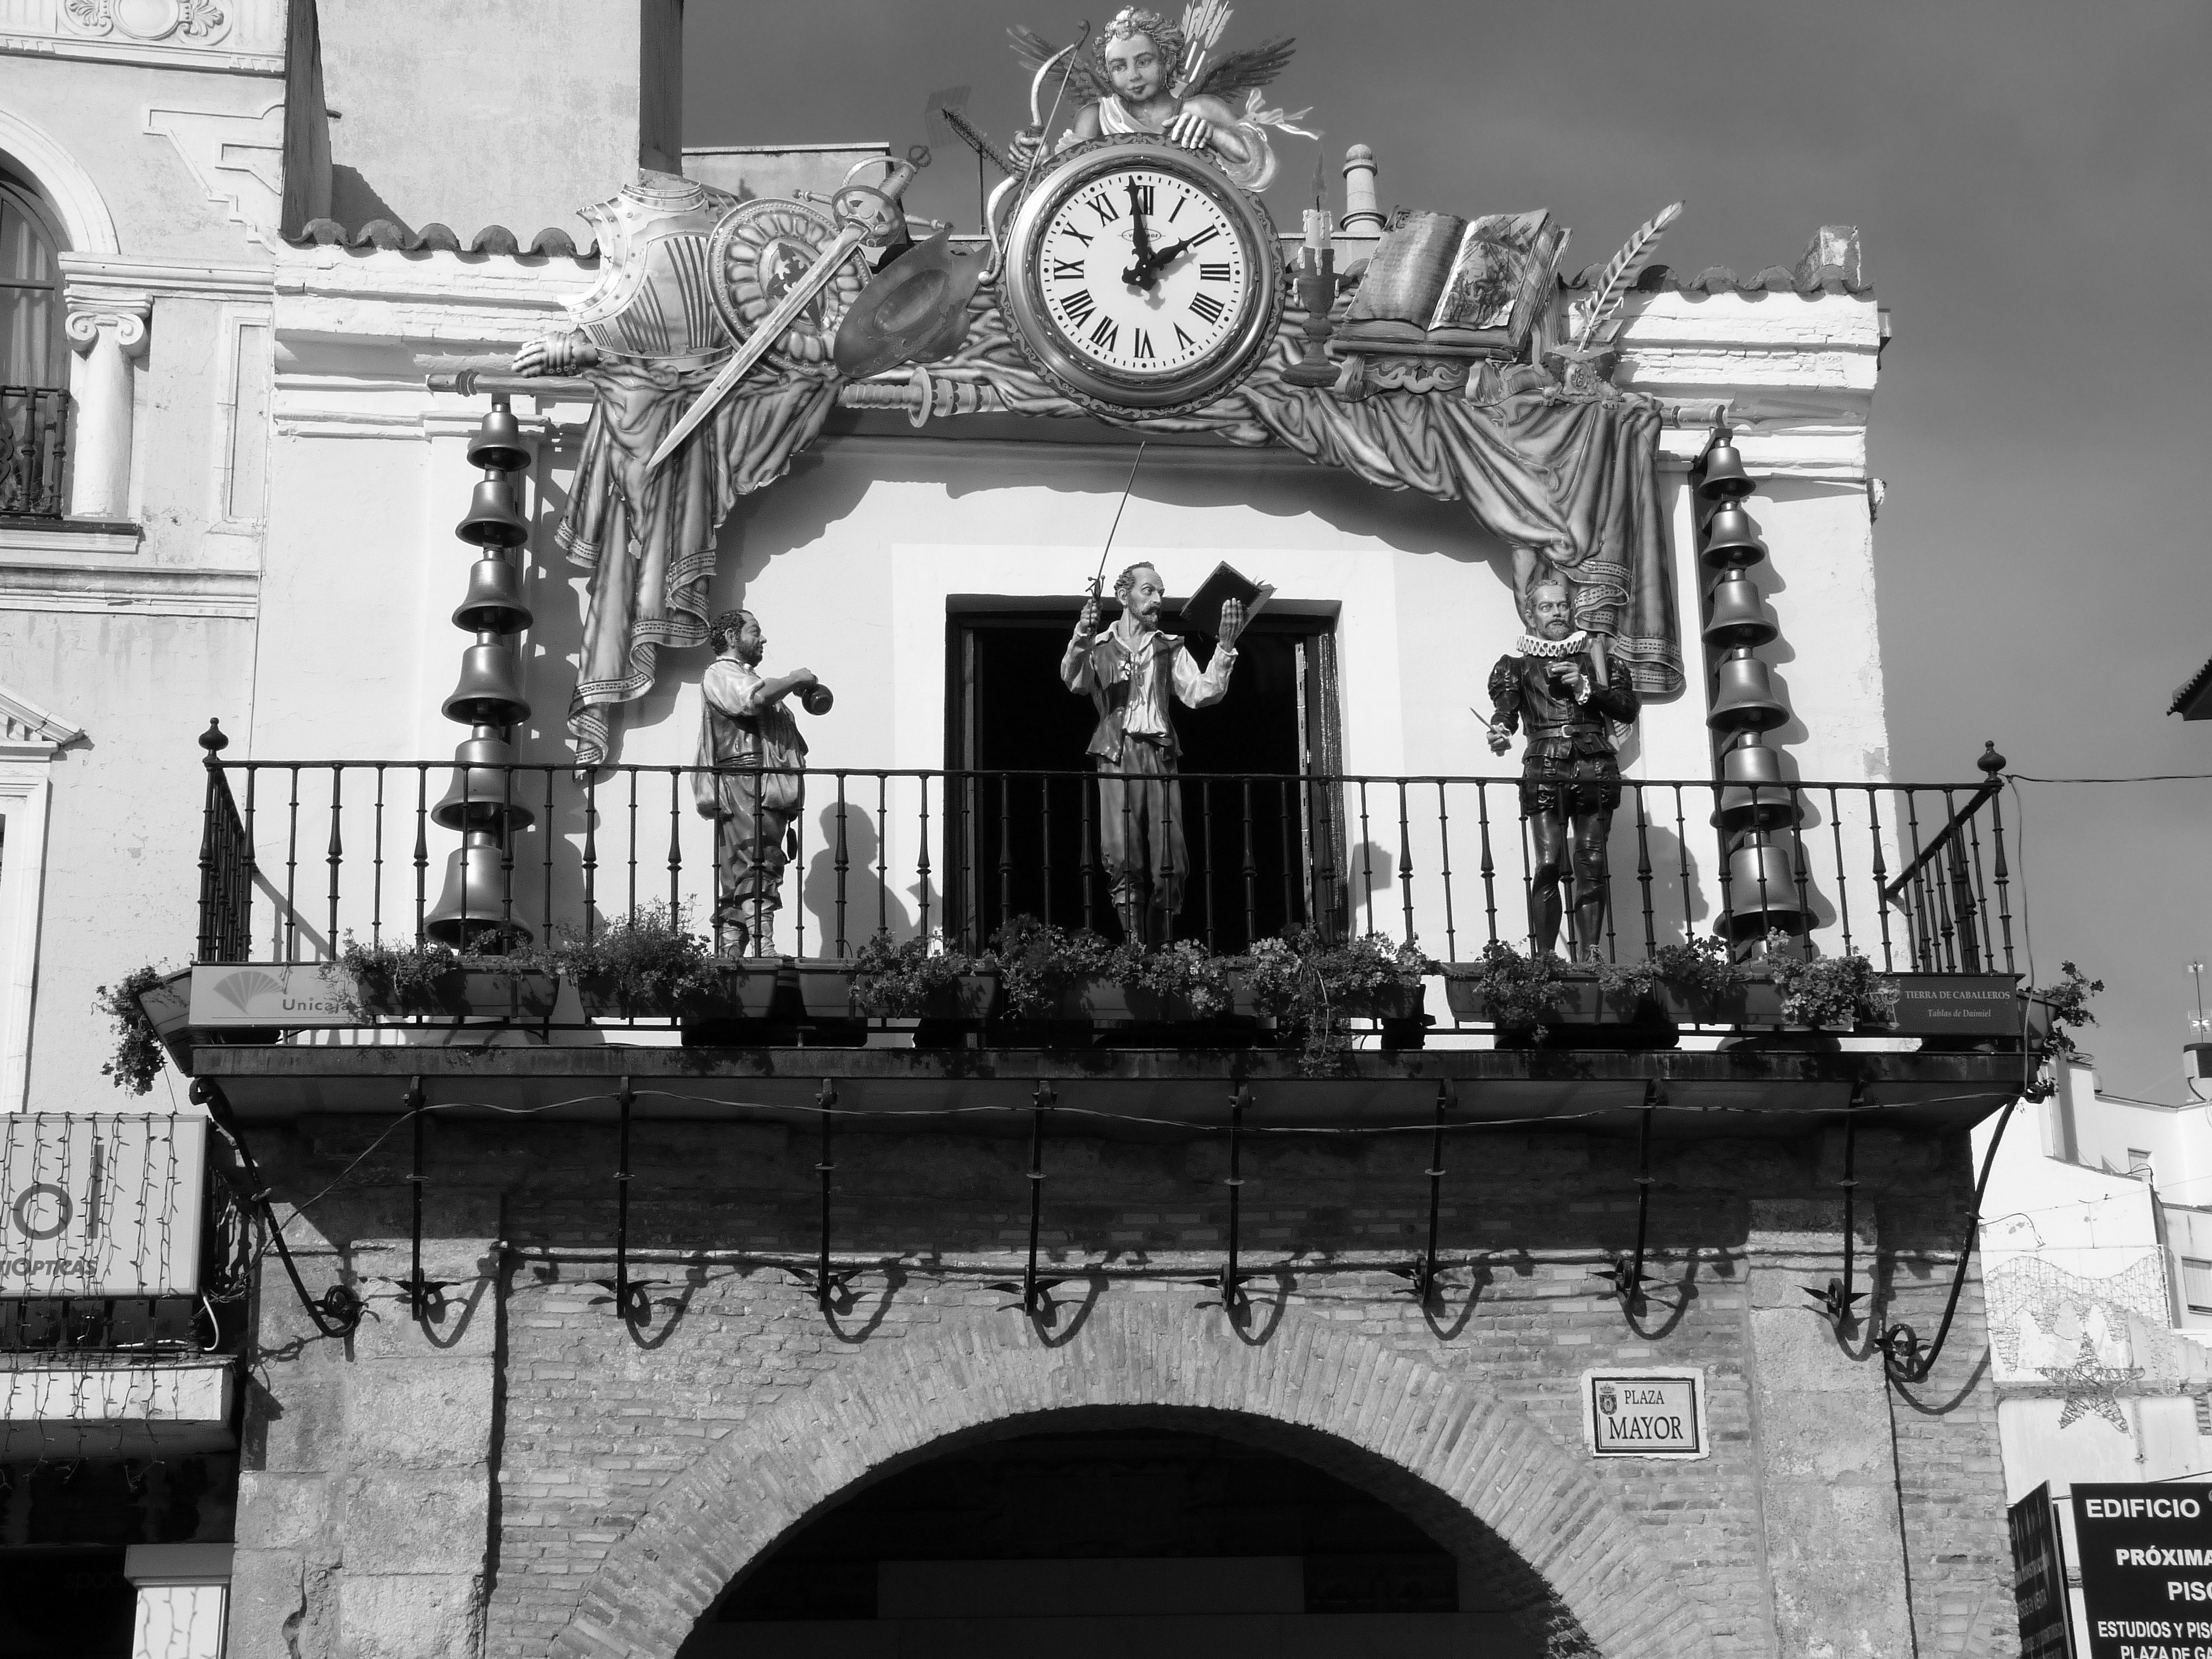
\includegraphics[width=0.8\linewidth]{./figs/clockCRbw}
		\caption{Fotografía en blanco y negro}\label{fig:fotoBW}
	\end{subfigure} 
	\caption[Ejemplo de subfiguras]{Ejemplo de inclusión de subfiguras en un mismo entorno (Fuente: J. Salido, \faCreativeCommons{} \faCreativeCommonsBy{} \faCreativeCommonsNcEu{} \faCreativeCommonsNd)}
	\label{fig:ejSubfigures}
\end{figure}

En los trabajos académicos la inclusión de imágenes y figuras que no son propiedad del autor suscitan bastante controversia, ya que con frecuencia se incumple inadvertidamente la ley vigente de propiedad intelectual. Respecto a este hecho se recomienda, tanto a estudiantes como tutores, consultar documentación informativa sobre el uso correcto de figuras en documentos académicos \cite{uclm20,unican18}. Entre las <<incorrecciones>> más habituales en los documentos académicos, se observa:
\begin{itemize}
\item \emph{Abuso del derecho de cita}. Se produce al incluir, con fines exclusivamente decorativos o ilustrativos de la explicación, una figura sujeta a derechos de uso restringido invocando el derecho de cita (incluso con correcta atribución de la obra).

\item \emph{Incorrecta atribución de la obra}. Es habitual confundir al autor de la obra con la fuente de origen de la misma. La fuente es precisa cuando se cita la obra original. Sin embargo, la licencia de muchas obras exige la atribución al autor y la inclusión de la licencia bajo la que se distribuye o hace uso de la misma (véase como ejemplo cómo se realiza una correcta atribución en las Fig.~\ref{fig:ejFigure} y \ref{fig:ejSubfigures} mencionando al autor y la licencia Creative-Commons\footnote{\url{https://creativecommons.org}} bajo la que se rige el uso de la imagen y el mecanismo de título alternativo para que dicha atribución no aparezca en el índice de figuras usando título opcional).

\item \emph{Supresión de los detalles de la licencia de uso}. Al incluir obras de terceros debemos tener presente los términos de distribución de la misma e incluirlos junto a la atribución de su legítimo autor.
\end{itemize}

La inclusión de material de \emph{dominio público}, sin restricciones de uso o con permiso, hace innecesaria la atribución al autor, pero se recomienda incluir una nota de agradecimiento.\footnote{Incluyendo un texto como: \emph{<<Por cortesía de ...>>}}

Cuando se presenta la necesidad de incluir un gráfico demasiado grande para el tamaño de la página, una opción muy apropiada es la impresión del gráfico en modo girado en una página aparte. Este efecto se consigue con el entorno \texttt{sidewaysfigure} proporcionado por el paquete \texttt{rotating}. La Fig.~\ref{fig:girada} muestra un ejemplo del entorno citado con un gráfico \textsf{PDF}.

\begin{sidewaysfigure}
	\centering
	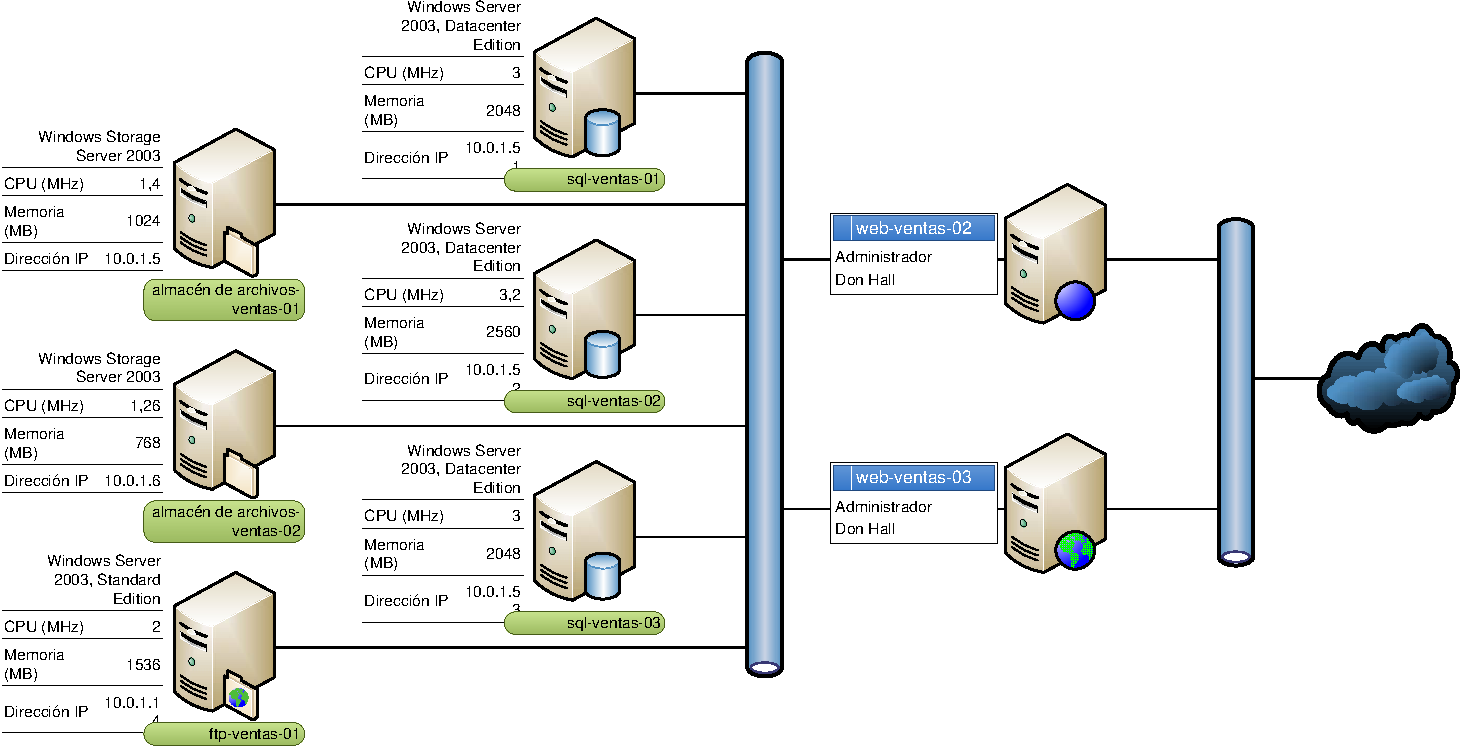
\includegraphics[width=0.98\textheight]{./figs/network} 
	\caption[Gráfico girado]{Figura vectorial con impresión girada}
	\label{fig:girada}
\end{sidewaysfigure}


\begin{landscape}
\thispagestyle{empty}
También es posible imprimir una página en formato apaisado cuando contiene una figura muy ancha. Este efecto se consigue con el paquete \texttt{pdflscape} y el entorno \texttt{landscape} proporcionado. Además, es este caso se han suprimido tanto la cabecera como el pie de página. La figura~\ref{fig:apaisada} se muestra apaisada a modo de ejemplo.

\begin{figure}[H]
	\centering
	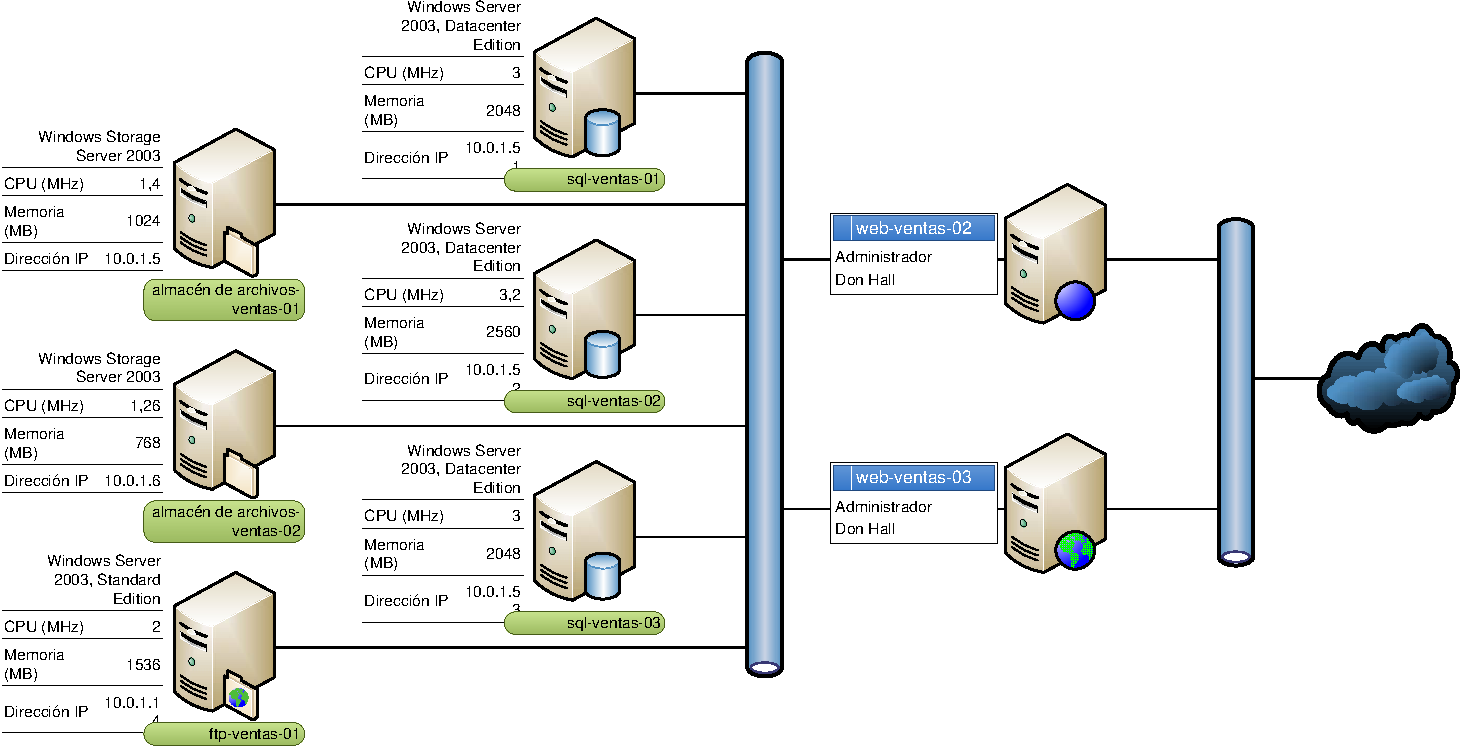
\includegraphics[width=\linewidth]{./figs/network} 
	\caption[Gráfico apaisado]{Figura vectorial con vista en página apaisada}
	\label{fig:apaisada}
\end{figure}
\end{landscape}


\section{Algoritmos y listados de código fuente}
En los textos científicos relacionados con las 
TIC\footnote{Por supuesto, en un TFG (Trabajo Fin de Grado) o tesis 
de un centro superior de Informática.} (Tecnologías de la Información y 
Comunicaciones) suelen aparecer porciones de código en los que se explica 
alguna función o característica relevante del trabajo que se expone. Muchas 
veces lo que se quiere ilustrar es un algoritmo o método con el que se resuelve un problema abstrayéndose del lenguaje de implementación. El paquete \texttt{algorithm2e} proporciona un entorno \texttt{algorithm} para la impresión apropiada de algoritmos, tratándolos como objetos flotantes y con mucha flexibilidad de personalización, como se observa en el algoritmo~\ref{alg:como} del ejemplo.


% Ejemplo:
% ============
\IncMargin{1em}
\begin{algorithm}
\SetKwInOut{Input}{Datos}\SetKwInOut{Output}{Resultado}
\LinesNumbered
\SetAlgoLined

\Input{este texto} 
%\KwIn{este texto}
\Output{como escribir algoritmos con \LaTeX2e}
%\KwOut{como escribir algoritmos con \LaTeX2e}

inicialización\;
\While{no es el fin del documento}{
	leer actual\;
	\eIf{comprendido}{
		ir a la siguiente sección\;
		la sección actual es esta\;
	}{
		ir al principio de la sección actual\;
	}
}

% Aunque el captión aparece abajo siempre se pone arriba como en tablas y listados
\caption{Cómo escribir algoritmos}\label{alg:como}
\end{algorithm}\DecMargin{1em}








\newpage % Añadido para visualizar los listados completos en una página.
La inclusión de porciones de código fuente se puede formatear de modo sencillo en \LaTeX{} mediante el uso del paquete \texttt{listings}. A continuación, se muestran varios ejemplos de porciones de código correspondientes a distintos lenguajes de programación.


% Ejemplo: Listado Java
% ============
% Los entornos lstlisting se pueden tratar tambión como elementos flotantes mediante la opción 'float=hbt', donde se indica la ubicación del elemento.
\begin{lstlisting}[language=Java,caption={[Código fuente en Java]Ejemplo de código fuente en lenguaje Java},label=lst:java]
// @author www.javadb.com
public class Main {    
// Este método convierte un String a un vector de bytes

public void convertStringToByteArray() {

String stringToConvert = "This String is 15";      
	byte[] theByteArray = stringToConvert.getBytes();        
	System.out.println(theByteArray.length);        
}

public static void main(String[] args) {
	new Main().convertStringToByteArray();
}
}
\end{lstlisting}


\begin{lstlisting}[style=ruled,language=C,caption={Ejemplo de código fuente en lenguaje C},label=lst:codC]
// Este código se ha incluido tal cual está en el fichero \LaTeX{}
#include <stdio.h>

int main(int argc, char* argv[]) {
	puts("¡Hola mundo!");
}
\end{lstlisting}


\begin{lstlisting}[style=ruled,language=Matlab,caption={Ejemplo de script en Matlab},label=lst:matlab]
function f = fibonacci(n)
% FIBONACCI  Fibonacci sequence
% f = FIBONACCI(n) generates the first n Fibonacci numbers.
%   Copyright 2014 Cleve Moler
% 	Copyright 2014 The MathWorks, Inc.

	f = zeros(n,1); 
	f(1) = 1;
	f(2) = 2;
	for k = 3:n
		f(k) = f(k-1) + f(k-2);
end
\end{lstlisting}



\section{Menús, paths y teclas con el paquete \texttt{menukeys}}
Cada vez es más usual que los trabajos en ingeniería exijan el uso de 
software. Para poder especificar de modo elegante el uso de menús, pulsaciones de teclas y directorios, se recomienda el uso del paquete 
\texttt{menukeys}.\footnote{\url{https://osl.ugr.es/CTAN/macros/latex/contrib/menukeys/menukeys.pdf}}
 \index{CTAN} Este paquete nos permite especificar el acceso a un menú, por 
ejemplo:

\noindent \menu{Herramientas:Órdenes:PDFLaTeX}

\noindent También un conjunto de teclas. Por ejemplo:
\keys{\ctrl + \shift + T}

\noindent O un directorio:
\directory{C:/user/LaTeX/Ejemplos}

\noindent Aunque este paquete permite muchas opciones de configuración de los estilos aplicados, esto no es necesario para obtener unos resultados muy elegantes.










 % Apéndice A (opcionales)

%END_FOLD
%--- (FIN DOCUMENTO)
\end{document}